%!TEX root = ../main.tex
% chktex-file 46
\chapter{Related Work}%
\label{sec:related}

Before combining \ac{lta} and \ac{gcr} as described in \cref{sec:intro:goals}, we first give an overview of the state-of-the-art in both fields of research.
This is done in three steps:
\begin{enumerate}
	\item We begin with an overview of the existing \ac{lta} methods for unstructured inputs.
	\item Then we look at the domain of structured inputs.
		To solve the \ac{gcr} problem, relevant graphs characteristics have to be defined in order to determine the similarity and dissimilarity of graphs.
		We will look at three approaches for graph characterization: The graph isomorphism test, the so-called \acl{wl} coloring and lastly the notion of graph spectra.W
	\item Based on the described graph characterization approaches, an overview of current \ac{gcr} methods will then be given.
\end{enumerate}

\section{Learning to Aggregate}%
\label{sec:related:lta}

The class of \ac{lta} problems was first described by \citet{Melnikov2016}.
There an input instance is understood as a composition $C = \ldblbrace c_1, \dots, c_n \rdblbrace$ of so-called constituents, i.e.\ as a variable-size multiset (denoted as $\ldblbrace \cdot \rdblbrace$).
The assumption in \ac{lta} problems is that for all constituents $c_i \in C$ a local score $y_i \in \mathcal{Y}$ is either given or computable.
The set of those local scores should be indicative of the overall score $y \in \mathcal{Y}$ of the composition $C$.
\ac{lta} problems typically require two subproblems to be solved:
\begin{enumerate}[label=\textbf{\arabic*.}]
	\item \textbf{Aggregation:}
		A variadic aggregation function $\mathcal{A}: \mathcal{Y}^{*} \to \mathcal{Y}$ that estimates composite scores has to be learned, i.e.\@ $y_i \approx \hat{y} = \mathcal{A}(y_{1}, \dots, y_{n})$.
		Typically the aggregation function $\mathcal{A}$ should be associative and commutative to fit with the multiset-structure of compositions.
	\item \textbf{Disaggregation:}
		In case the constituent scores $y_i$ are not given, they have to be derived from a constituent representation, e.g.\ a vector $x_i \in \mathcal{X}$.
		To learn this derivation function $f: \mathcal{X} \to \mathcal{Y}$, only the constituent vectors ${\ldblbrace x_i \rdblbrace}_{i = 1}^{n}$ and the composite score $y$ is given.
		Thus the constituent scores $y_i$ need to be \textit{disaggregated} from $y$ in order to learn $f$.
\end{enumerate}
\begin{figure}[ht]
	\centering
	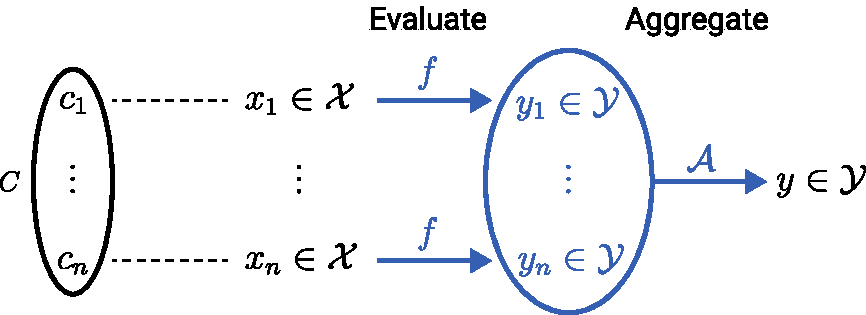
\includegraphics[width=0.7\linewidth]{gfx/related-work/lta-overview.pdf}
	\caption{Overview of the structure of LTA for multiset compositions.}\label{fig:related:lta-overview}
\end{figure}
Overall \ac{lta} can be understood as the joint problem of learning the aggregation function $\mathcal{A}$ and the local score derivation function $f$.
Two main approaches to represent the aggregation function in \ac{lta} problems have been explored.

\subsection{Uninorm-Aggregation}%
\label{sec:related:lta:uninorm}

The first approach uses \textit{uninorms}~\cite{Melnikov2016} to do so.
There the basic idea is to express composite scores as fuzzy truth assignments $y \in [0, 1]$.
Such a composite assignment $y$ is modeled as the result of a parameterized logical expression of constituent assignments $y_i \in [0, 1]$.
As the logical expression that thus effectively aggregates the constituents, a uninorm $U_{\lambda}$ is used.
Depending on the parameter $\lambda \in [0, 1]$, $U_{\lambda}$ combines a t-norm $T$ and a t-conorm $S$ which are continuous generalizations of logical conjunction and disjunction respectively.
One popular choice of norms are the so-called Łukasiewicz norms:
\begin{align}
	\text{t-norm } T(a, b) &\coloneqq \max \{ 0, a + b - 1 \}, \quad\text{t-conorm } S(a, b) \coloneqq \min \{ a + b, 1 \}, \nonumber \\
	\text{uninorm } U_\lambda(a, b) &\coloneqq \begin{cases}
		\lambda T\left(\frac{a}{\lambda}, \frac{b}{\lambda}\right) & \text{if } a, b \in [0, \lambda] \\
		\lambda + (1 - \lambda) S\left(\frac{a - \lambda}{1 - \lambda}, \frac{b - \lambda}{1 - \lambda}\right) & \text{if } a, b \in [\lambda, 1] \\
		\lambda \min \{ a, b \} & \text{else}
	\end{cases}
\end{align}
At the extreme points $(0, 0)$, $(0, 1)$, $(1, 0)$ and $(1, 1)$, $T$ and $S$ coincide with the Boolean operators $\land$ and $\lor$;
the values at all other points are interpolated as shown in \cref{fig:related:logic-norms}.
The uninorm $U_\lambda$ uses the conjunctive t-norm $T$ for values below the threshold $\lambda$ and the disjunctive t-conorm $S$ for values above the threshold.
$U_\lambda$ therefore smoothly interpolates between a conjunctive and disjunctive operator with the extreme points $U_1 = T$ and $U_0 = S$.
\begin{figure}[ht]
	\centering
	\begin{tikzpicture}
		\begin{axis}[
			title={t-norm $T$ ($\land$)},
			xlabel=$a$,
			ylabel=$b$,
			xlabel style={xshift=0.2cm, yshift=0.15cm},
			ylabel style={xshift=-0.2cm, yshift=0.15cm},
			tick label style={font=\scriptsize},
			width=0.33\textwidth,
			colormap = {bluered}{color(0cm) = (t_blue); color(1cm) = (t_red)}
		]
			\addplot3[
				mesh,
				samples=12,
				domain=0:1,
				domain y=0:1
			]{max(x + y - 1, 0)};
		\end{axis}
	\end{tikzpicture}
	\begin{tikzpicture}
		\begin{axis}[
			title={t-conorm $S$ ($\lor$)},
			xlabel=$a$,
			ylabel=$b$,
			xlabel style={xshift=0.2cm, yshift=0.15cm},
			ylabel style={xshift=-0.2cm, yshift=0.15cm},
			tick label style={font=\scriptsize},
			width=0.33\textwidth,
			colormap = {bluered}{color(0cm) = (t_blue); color(1cm) = (t_red)}
		]
			\addplot3[
				mesh,
				samples=12,
				domain=0:1,
				domain y=0:1
			]{min(x + y, 1)};
		\end{axis}
	\end{tikzpicture}
	\begin{tikzpicture}
		\begin{axis}[
			title={uninorm $U_{0.5}$ ($\land$/$\lor$)},
			xlabel=$a$,
			ylabel=$b$,
			xlabel style={xshift=0.2cm, yshift=0.15cm},
			ylabel style={xshift=-0.2cm, yshift=0.15cm},
			tick label style={font=\scriptsize},
			width=0.33\textwidth,
			colormap = {bluered}{color(0cm) = (t_blue); color(1cm) = (t_red)}
		]
			\addplot3[
				mesh,
				samples=12,
				domain=0:1,
				domain y=0:1
			]{(x <= 0.5 && y <= 0.5) * 0.5 * max(2 * (x + y) - 1, 0) + (x > 0.5 && y > 0.5) * (0.5 + 0.5 * min(2 * (x + y - 1), 1)) + (!(x <= 0.5 && y <= 0.5) && !(x > 0.5 && y > 0.5)) * min(x, y)};
		\end{axis}
	\end{tikzpicture}
	\caption{The Łukasiewicz norms and the corresponding uninorm for $\lambda = 0.5$.}\label{fig:related:logic-norms}
\end{figure}

Since t-norms and t-conorms are commutative and associative they can also be applied to non-empty sets of arbitrary size, i.e. $T(\ldblbrace y_1, \dots, y_n \rdblbrace) = T(y_1, T(\ldblbrace y_2, \dots, y_n \rdblbrace))$ with fixpoint $T(\ldblbrace y \rdblbrace) = y$.
Using this extension, a uninorm $U_\lambda$ can be applied to sets which turns it into a parameterized aggregation function $\mathcal{A}_\lambda: {[0, 1]}^* \to [0, 1]$.
In this simple model the \ac{lta} aggregation problem boils down to the optimization of $\lambda$.
The \ac{lta} disaggregation problem is solved by jointly optimizing a \acl{lm}, i.e.\ the constituent scores ${\ldblbrace y_i \in [0, 1] \rdblbrace}_{c_i \in C}$ are described by $y_i = {\left( 1 + \exp(-\theta^\top x_i) \right)}^{-1}$.
Overall an \ac{lta} model is therefore described by the uninorm parameter $\lambda$ and the regression coefficients $\theta$.

\subsection{\acs*{owa}-Aggregation}%
\label{sec:related:lta:owa}

Recently \citet{Melnikov2019} have looked at an alternative class of aggregation functions.
Instead of using fuzzy logic to describe score aggregation, \ac{owa} operators were used.
\ac{owa} aggregators work by sorting the input scores and then weighting them based on their sort position, i.e.\ %
\begin{align}
	\mathcal{A}_{\lambda}(y_1, \dots, y_n) \coloneqq \sum_{i = 1}^n \lambda_i y_{\pi(i)},
\end{align}
where $\lambda \in \mathbb{R}^n$ is a weight vector with ${\|\lambda\|}_1 = 1$ and $\pi: [n] \to [n]$ is a sorting permutation of the input scores with $[n] \coloneqq \{ 1, \dots, n \}$ and $y_i < y_j \Rightarrow \pi(i) < \pi(j)$. % chktex 21
Depending on the choice of the vector $\lambda$, the \ac{owa} function $\mathcal{A}_\lambda$ can express common aggregation functions like
$\min$ (if $\lambda = (1, 0, \dots, 0)$),
$\max$ (if $\lambda = (0, \dots, 0, 1)$)
or the arithmetic mean (if $\lambda = \left(\frac{1}{n}, \dots, \frac{1}{n}\right)$).

To deal with varying composition sizes $n$, the weights $\lambda_1, \dots, \lambda_n$ can however not be statically assigned.
Instead they are interpolated using a so-called \ac{bum} function $q: [0, 1] \to [0, 1]$.
It takes constituent positions that are normalized to the unit interval, i.e.\ $\frac{i}{n} \in [0, 1]$.
The \ac{bum} function $q$ is then used to interpolate a weight for any normalized sort position via $\lambda_i \coloneqq q\left(\frac{i}{n}\right) - q\left(\frac{i - 1}{n}\right)$.
Because $q$ is monotone with $q(0) = 0$ and $q(1) = 1$, it always holds that ${\|\lambda\|}_1 = q(1) - q(0) = 1$. % chktex 21
Using this model, the aggregation problem boils down to optimizing the shape of $q$.

\begin{figure}[ht]
	\centering
	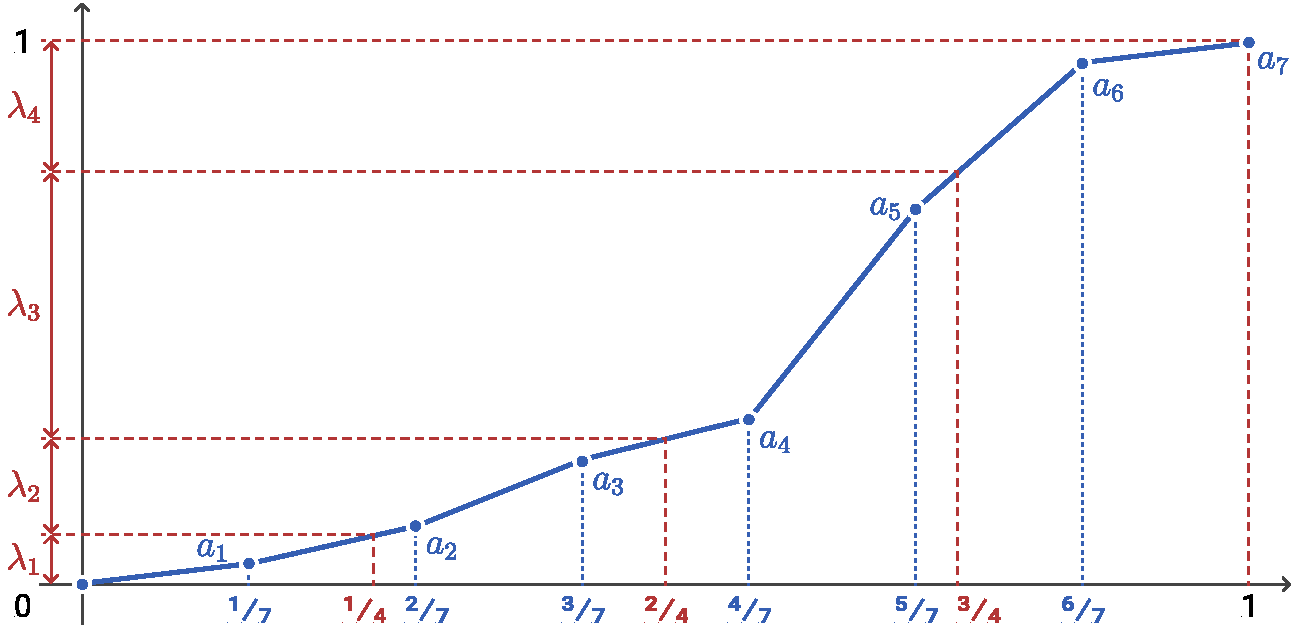
\includegraphics[width=0.72\linewidth]{gfx/related-work/bum.pdf}
	\caption[Illustration of how a \ac{bum} function is described as a linear spline and its relation to the \ac{owa} weights.]{
		Illustration of how \textcolor{t_blue}{$a$} describes \textcolor{t_blue}{$q$} and its relation to \textcolor{t_red}{$\lambda$} ($n = 4$, $m = 7$).
	}\label{fig:related:bum}
\end{figure}
In the \ac{owa} approach the \ac{bum} function $q$ is modeled as a piecewise linear spline.
This spline is described by $m+1$ points ${\left\{ \left( \frac{j}{m}, a_j \right) \right\}}_{j = 0}^{m}$, the so-called knots of the spline. % chktex 21
The curve of $q$ is obtained by linearly interpolating between neighboring knots as shown in \cref{fig:related:bum}.
If $0 = a_0 \leq a_1 \leq \cdots \leq a_m = 1$, $q$ is a \ac{bum} function.
The \ac{lta} aggregation problem is therefore solved by optimizing $a \in \mathbb{R}^{m + 1}$ under this constraint.
The disaggregation problem is tackled by adding the scores $y_1, \dots, y_M \in \mathbb{R}$ to the learnable parameters of the model where $M$ is assumed to be the finite number of constituents.
Currently the \ac{owa} approach requires all possible constituents to be part of the training dataset since it does not consider constituent features $x_i \in \mathcal{X}$ to predict the scores of previously unseen constituents.

\section{Graph Characterization}%
\label{sec:related:character}

\begin{defn}
	A \textit{graph} $G \coloneqq (\mathcal{V}_G, \mathcal{E}_G)$ consists of a finite set of vertices $v_i \in \mathcal{V}_G$ and a set of edges $e_{ij} = (v_i, v_j) \in \mathcal{E}_G \subseteq \mathcal{V}_G^2$.
	Optionally discrete vertex labels $l_G[v_i] \in L_{\mathcal{V}}$ or edge labels $l_G[e_{ij}] \in L_{\mathcal{E}}$ may be associated with all vertices $v_i \in \mathcal{V}_G$ and edges $e_{ij}\in \mathcal{E}_G$ respectively.
	Also continuous feature vectors $x_G[v_{i}] \in \mathcal{X}_{\mathcal{V}}$, $x_G[e_{ij}] \in \mathcal{X}_{\mathcal{E}}$ may be given.
	If $\mathcal{X}_{\mathcal{E}} = \mathbb{R}$, $x_G[e_{ij}]$ can be interpreted as an edge weight of $e_{ij}$.

	In this thesis all graphs $G$ are assumed to be undirected if not explicitly stated otherwise, i.e.\ ${e_{ij} \in \mathcal{E}_G} \leftrightarrow\allowbreak {e_{ji} \in \mathcal{E}_G} \allowbreak\land l_G[e_{ij}] = l_G[e_{ji}] \allowbreak\land x_G[e_{ij}] = x_G[e_{ji}]$.
	We denote the set of all undirected graphs as $\mathcal{G}$.
	Additionally we denote $G[S] \coloneqq (S, \mathcal{E}_G \cap S^2)$ as the subgraph of $G$ induced by $S \subseteq \mathcal{V}_G$.
\end{defn}
To classify or score a graph, it first needs to be characterized by a set of relevant properties.
The most strict characterization of a graph is its so-called \textit{isomorphism class}.
It uniquely identifies a graph but lacks any notion of similarity between non-identical graphs.
We will begin with a brief definition of this strict isomorphism-based graph characterization.
Then two less strict characterization approaches are described; the so called \acl{wl} coloring and the notion of graph spectra.
They are the theoretical foundation of many current \ac{gcr} methods.

\subsection{The Graph Isomorphism Problem}%
\label{sec:related:character:iso}

In order to process a graph $G$ of size $n = |\mathcal{V}_G|$, one is forced to choose some encoding, e.g.\ an adjacency matrix $A_G \in {\{0, 1\}}^{n \times n}$.
Such an encoding introduces a vertex ordering $v_1, \dots, v_n$ that does not carry any semantic meaning.
Consequently there are $n!$ equivalent encodings of $G$. % chktex 40
To represent those encodings we introduce the notion of ordered induced subgraphs.
\begin{defn}\label{defn:related:ordered-subgraph}
	For all vertex $k$-tuples $v = (v_1, \dots, v_k) \in \mathcal{V}_G^k$ let $\hat{v} = \{ v_i\, |\, i \in [k] \}$.
	Then $G[v] \coloneqq (\hat{v}, \mathcal{E}_G \cap \hat{v}^2, v)$ is called the \textit{ordered subgraph} of $G$ induced by $v$.
	If $\hat{v} = \mathcal{V}_G$ and $k = |\mathcal{V}_G|$, we call $v$ an \textit{ordering} of $G$ and $G[v]$ an \textit{encoding} of $G$.
\end{defn}
\begin{defn}\label{defn:related:ordered-subgraph-equivalence}
	Two ordered induced subgraphs $G[v]$ and $H[w]$ with $(v_1, \dots, v_k) \in \mathcal{V}_G^k$ and $(w_1, \dots, w_k) \in \mathcal{V}_H^k$ are \textit{equivalent} ($G[v] \equiv H[w]$) iff.\
	\begin{align*}
		&\quad\forall i, j \in [k]: (v_i, v_j) \in \mathcal{E}_G \leftrightarrow (w_i, w_j) \in \mathcal{E}_H \\
		&\, \begin{aligned}
			\land&\ \forall i, j \in [k]: l_G[v_i, v_j] = l_H[w_i, w_j] &\land&\quad\forall i \in [k]: l_G[v_i] = l_H[w_i] \\
			\land&\ \forall i, j \in [k]: x_G[v_i, v_j] = x_H[w_i, w_j] &\land&\quad\forall i \in [k]: x_G[v_i] = x_H[w_i]\text{.}
		\end{aligned}
	\end{align*}
	Using this notion of equivalence, we call ${\left[ G[v] \right]} \coloneqq \{ G[w]\, |\, G[w] \equiv G[v] \land w \in \mathcal{V}_G^{*} \}$ the \textit{ordered subgraph equivalence class} of $G[v]$.
\end{defn}
\begin{defn}
	Two graphs $G$ and $H$ are \textit{isomorphic} ($G \simeq H$) iff.\ there are equivalent encodings $G[v] \equiv H[w]$ of them.
	Consequently $[G] \coloneqq \{ H\, |\, H \simeq G \}$ is called the \textit{isomorphism class} of $G$.
\end{defn}
The goal of the \ac{gi} problem is to check whether $G \simeq H$ for two arbitrary graphs.
Even though there is no known universal polynomial algorithm that solves \ac{gi}, \citet{Babai1980} showed that almost all graphs can be trivially distinguished in linear time.
More recently \citet{Babai2015} also presented a quasipolynomial upper time bound for the remaining hard \ac{gi} instances.
For all practical purposes, \ac{gi} can therefore be solved efficiently; e.g.\ via the \texttt{nauty} program~\cite{McKay}\cite{McKay2013}.
One important subroutine in most \ac{gi} checkers is the \acl{wl} algorithm which will be described next.

\subsection{\acl{wl} Graph Colorings}%
\label{sec:related:character:wl}

The \acf{wl} algorithm~\cite{Weisfeiler1968}\cite{Cai1992} characterizes a graph $G$ by assigning discrete labels $c \in \mathcal{C}$, called \textit{colors}, to vertex $k$-tuples $(v_1, \dots, v_k) \in \mathcal{V}_G^k$, where $k \in \mathbb{N}$ is the freely choosable \textit{\ac{wl}-dimension}.
A mapping $\chi_{G, k}: \mathcal{V}_G^k \to \mathcal{C}$ is called a \textit{$k$-coloring} of $G$.
\begin{defn}
	A coloring $\chi'$ \textit{refines} $\chi$ ($\chi' \preceq \chi$) iff.\ $\forall a, b \in \mathcal{V}_G^k: \chi(a) \neq \chi(b) \rightarrow \chi'(a) \neq \chi'(b)$, i.e.\ $\chi'$ distinguishes at least those tuples that are distinguished by $\chi$.
\end{defn}
\begin{defn}
	Two colorings $\chi$ and $\chi'$ are \textit{equivalent} ($\chi \equiv \chi'$) iff.\ $\chi \preceq \chi' \land \chi \succeq \chi'$, i.e.\ $\chi$ is identical to $\chi'$ up to color substitutions.
\end{defn}
The $k$-dimensional \ac{wl} algorithm ($k$-\acs{wl}) works by iteratively refining $k$-colorings $\chi_{G, k}^{(0)} \succeq \chi_{G, k}^{(1)} \succeq \dots$ of a given graph $G$ until the convergence criterion $\chi_{G, k}^{(i)} \equiv \chi_{G, k}^{(i+1)}$ is satisfied.
We denote the final, maximally refined $k$-\acs{wl} coloring with $\chi^{*}_{G, k}$.
\begin{defn}
	The color distribution $\mathit{dist}_{\chi_{G, k}}: \mathcal{C} \to \mathbb{N}$ of a $k$-coloring $\chi_{G, k}$ counts each color $c \in \mathcal{C}$ in the coloring, i.e.\ $\mathit{dist}_{\chi_{G, k}}(c) \coloneqq \left|\left\{ v \in \mathcal{V}_G^k\, |\, \chi_{G, k}(v) = c \right\}\right|$. % chktex 21
\end{defn}
\begin{defn}\label{defn:related:wl-distinguishable}
	Two graphs $G$ and $H$ are $k$-\acs{wl} \textit{distinguishable} ($G \mathrel{{\not\simeq}_k} H$) iff.\ there exists a color $c \in \mathcal{C}$ s.t.\ $\mathit{dist}_{\chi^{*}_{G, k}}(c) \neq \mathit{dist}_{\chi^{*}_{H, k}}(c)$.
\end{defn}
As we will see, the way in which \ac{wl} colorings are refined is vertex order invariant;
thus any difference in the final coloring of two graphs always implies the non-isomorphism of the colored graphs, i.e.\ $G \mathrel{{\not\simeq}_k} H \implies G \not\simeq H$.
The opposite does however not necessarily hold;
two $k$-\acs{wl} indistinguishable graphs are not always isomorphic, i.e.\ $\exists\, G, H: G \mathrel{{\simeq}_k} H \land G \not\simeq H$. % chktex 21

In addition to the binary aspect of \ac{wl} distinguishability and its relation to the \ac{gi} problem, \ac{wl} colorings are also useful for more fuzzy graph similarity comparisons as we will see in \cref{sec:related:gcr:kernel} when we look at graph kernels.
Before that however, the details of \ac{wl} color refinement strategy have to be described.
We begin with the color refinement algorithm for the most simple case of $k = 1$.
Then the definitions and intuitions from the 1-dimensional case are extended to its higher-dimensional generalization.
Lastly we will discuss the discriminative power of the \acs{wl} algorithm and its relation to the \acs{wl}-dimension $k$.

\subsubsection{The 1-dimensional \acs{wl} algorithm}
In the 1-dimensional \ac{wl} algorithm (1-WL), a color is assigned to each vertex of a graph.
If the vertices $v \in \mathcal{V}_G$ of the input graph $G$ are labeled, those labels $l_G[v] \in L_{\mathcal{V}} \subseteq \mathcal{C}$ can be used as the initial graph coloring $\chi_{G,1}^{(0)}(v) \coloneqq l_G[v]$.
Since \ac{wl} colors are inherently discrete, continuous vertex feature vectors $x_G[v]$ are not considered here.
For unlabeled graphs a constant coloring is used, e.g.\ $\forall v \in \mathcal{V}_G: \chi_{G,1}^{(0)}(v) = \textcolor{t_blue}{\texttt{A}}$ for some initial color $\textcolor{t_blue}{\texttt{A}} \in \mathcal{C}$. % chktex 25
In each iteration of the 1-\acs{wl} color refinement algorithm, the following neighborhood aggregation scheme is used to compute a new color for all vertices:
\begin{defn}\label{defn:related:wl1-refine}
	$\chi_{G,1}^{(i+1)}(v) \coloneqq h\left(\chi_{G,1}^{(i)}(v), \ldblbrace \chi_{G,1}^{(i)}(u)\, |\, u \in \Gamma_{G}(v) \rdblbrace\right)$,
	with $\Gamma_G(v)$ denoting the set of adjacent vertices of $v \in \mathcal{V}_G$ and $h: \mathcal{C}^* \to \mathcal{C}$ denoting an injective hash function that assigns a unique color to each finite combination of colors.
\end{defn}
\begin{figure}[ht]
	\centering
	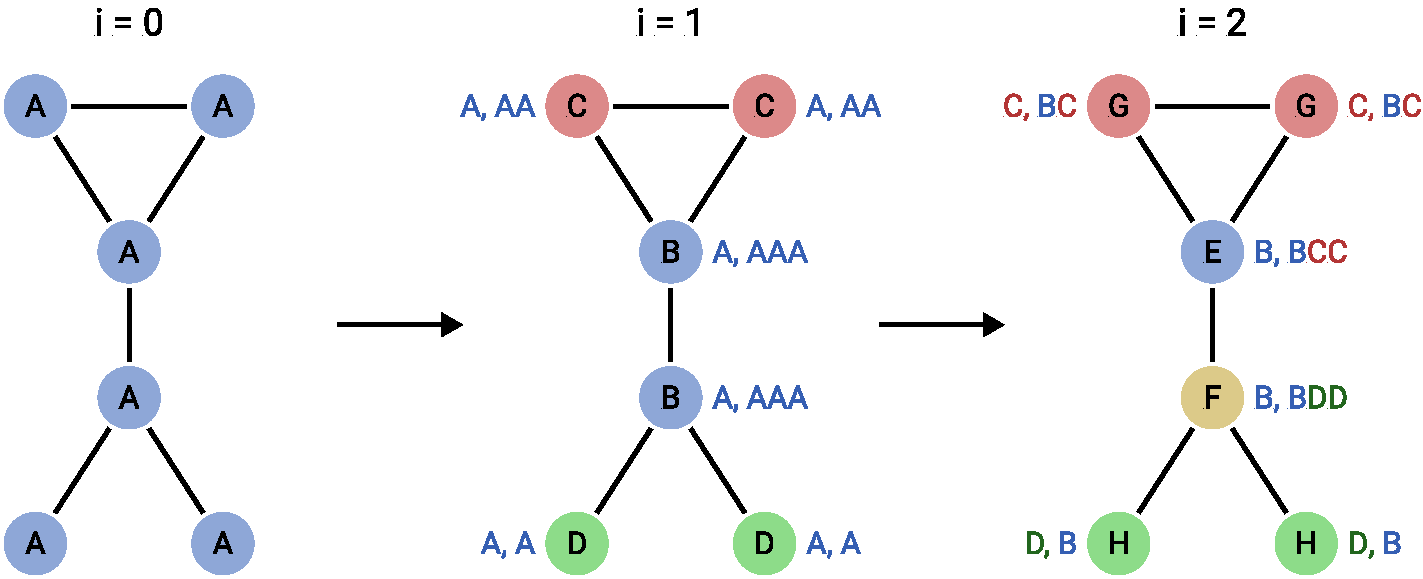
\includegraphics[width=0.72\linewidth]{gfx/related-work/wl1-refine.pdf}
	\caption[Example 1-WL color refinement steps.]{
		Example 1-WL color refinement steps.
		After two iterations the coloring stabilizes.
		Each vertex $v$ is labeled with its current color and has its previous color and the colors of the hashed neighbors $\Gamma_G(v)$ written next to it (see \cref{defn:related:wl1-refine}).
	}\label{fig:related:wl1-refine}
\end{figure}
In practice the hash function $h$ is usually defined lazily by using $\mathcal{C} \subseteq \mathbb{N}$ and enumerating color combinations in whichever order they are hashed s.t.\ a new color is introduced every time a previously unseen color combination appears at runtime\footnote{
	Note that, even though $\mathcal{C}$ is formally countably infinite, we will assume that it only contains the finite number of colors occurring in a given finite graph dataset.
}.

\subsubsection{The $k$-dimensional \acs{wl} algorithm}
As we just saw, the 1-\acs{wl} algorithm iteratively refines colorings of single vertices.
While the obtained colorings differ for most non-isomorphic graphs $G \not\simeq H$, 1-\acs{wl} does not generally solve the \ac{gi} problem as illustrated in \cref{fig:related:wl1-problem}.
\begin{figure}[ht]
	\centering
	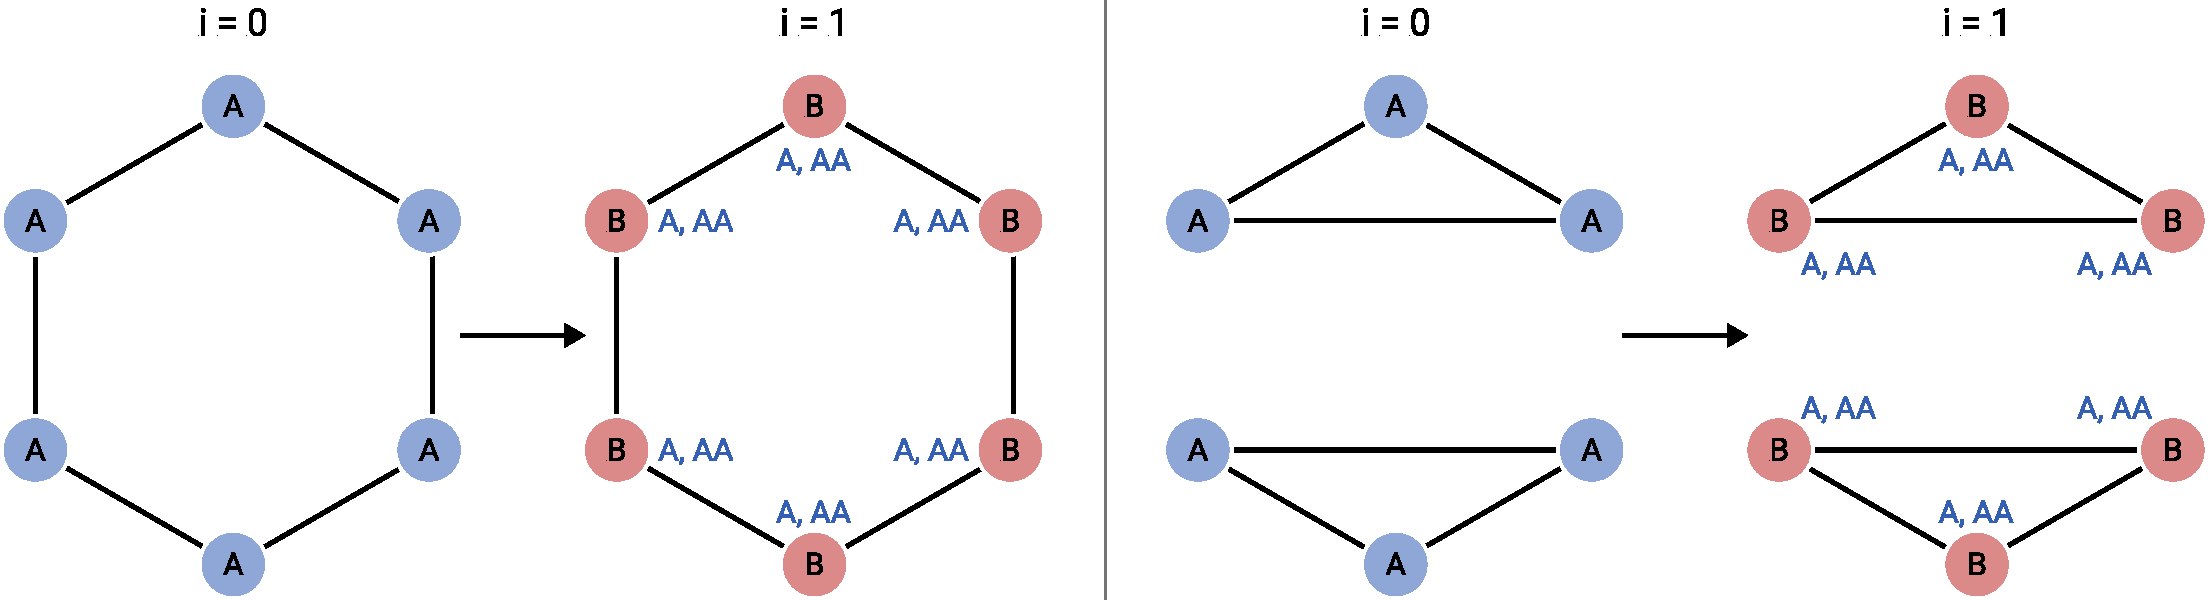
\includegraphics[width=\linewidth]{gfx/related-work/wl1-problem.pdf}
	\caption[Two simple non-isomorphic graphs that are indistinguishable by 1-\acs{wl}.]{
		Two simple non-isomorphic graphs that are indistinguishable by 1-\acs{wl}.
	}\label{fig:related:wl1-problem}
\end{figure}\\
By extending \ac{wl} to higher dimensions, such 1-\acs{wl} indistinguishable cases can however be handled.
Analogous to the 1-dimensional \cref{defn:related:wl1-refine}, the $k$-dimensional color refinement step is defined by
\begin{defn}\label{defn:related:wlk-refine}
	$\begin{aligned}[t]
		\chi_{G,k}^{(i+1)}(s) \coloneqq h\left(\chi_{G,k}^{(i)}(s), \ldblbrace (\chi_{G,k}^{(i)}(s[u/1]), \dots, \chi_{G,k}^{(i)}(s[u/k]))\, |\, u \in \mathcal{V}_G \rdblbrace\right)\\
		\text{with } s = (v_1, \dots, v_k) \in \mathcal{V}_G^k,\quad s[u/j] \coloneqq (v_1, \dots, v_{j-1}, u, v_{j+1}, \dots, v_k) \text{.}
	\end{aligned}$
\end{defn}
In 1-\acs{wl} a vertex color is refined by combining the colors of neighboring vertices.
In $k$-\acs{wl} the color of a $k$-tuple $s \in \mathcal{V}_G^k$ is refined by combining the colors of its neighborhood which is defined as the set of all $k$-tuples in which at most one vertex differs from $s$.
Note that each vertex $k$-tuple has one neighbor for each $u \in \mathcal{V}_G$, each of which is a $k$-tuple of vertex $k$-tuples.
This more abstract notion of neighborhood is illustrated in \cref{fig:related:wl-neighbors}.
\begin{figure}[ht]
	\centering
	\begin{subfigure}{0.33\textwidth}
		\centering
		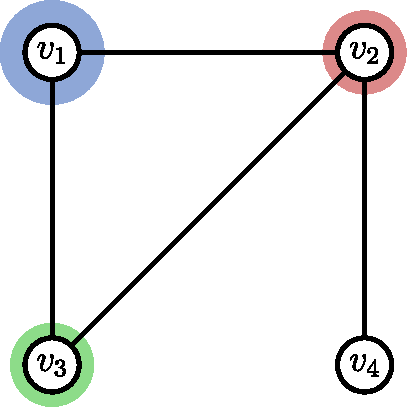
\includegraphics[width=0.8\linewidth]{gfx/related-work/wl1-neighbors.pdf}
		\subcaption{1-WL $v_1$ neighbors}\label{fig:related:wl-neighbors:1}
	\end{subfigure}%
	\begin{subfigure}{0.33\textwidth}
		\centering
		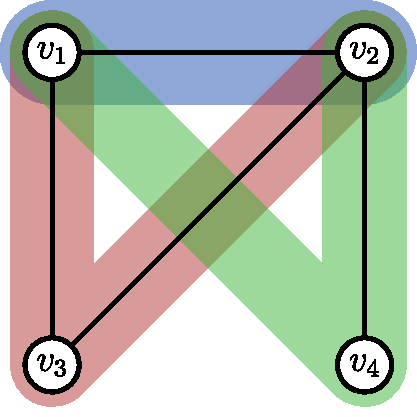
\includegraphics[width=0.8\linewidth]{gfx/related-work/wl2-neighbors.pdf}
		\subcaption{2-WL $(v_1, v_2)$ neighbors}\label{fig:related:wl-neighbors:2}
	\end{subfigure}%
	\begin{subfigure}{0.33\textwidth}
		\centering
		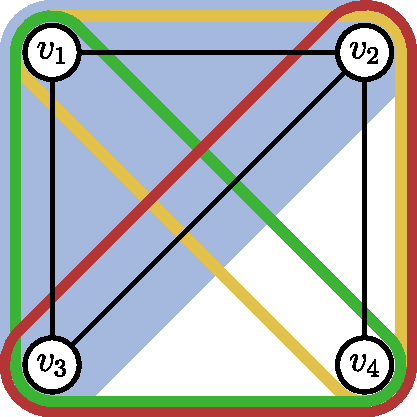
\includegraphics[width=0.8\linewidth]{gfx/related-work/wl3-neighbors.pdf}
		\subcaption{3-WL $(v_1, v_2, v_3)$ neighbors}\label{fig:related:wl-neighbors:3}
	\end{subfigure}
	\caption[\ac{wl} neighborhoods for different values of $k$.]{
		Tuple neighborhoods for different values of $k$.
		The vertices highlighted in \textcolor{t_blue}{blue} form the root tuple $s \in \mathcal{V}_G^k$ whose neighbors are shown;
		for simplicity neighbors with $u \in s$ are left out (see~\cref{defn:related:wlk-refine}).
		Each neighbor is highlighted with a different color, except for 3-WL where the \textcolor{t_red}{red}, \textcolor{t_darkgreen}{green} and \textcolor{t_darkyellow}{yellow} triples actually form the single neighbor for $u = v_4$.
	}\label{fig:related:wl-neighbors}
\end{figure}
For $k = 2$ this means that each potential edge $(v, w) \in \mathcal{V}_G^2$ has all possible paths of length $2$ from $v$ to $w$ as its neighbors (see~\cref{fig:related:wl-neighbors:2}).
Also note that, even though $k$-\acs{wl} refines $k$-tuple colors, lower-dimensional structures still get their own colors since a tuple does not have to consist of distinct vertices, i.e.\ in $k$-\acs{wl} the color of a single vertex $v \in \mathcal{V}_G$ is described by $\chi^{*}_{G, k}(s)$ for $s = (v, \dots, v) \in \mathcal{V}_G^k$.

Let us now look at how the tuple colors are initialized.
For this we use the ordered subgraph equivalence classes $[G[s]]$ (see~\cref{defn:related:ordered-subgraph-equivalence}) which determine the initial color $\chi_{G,k}^{(0)}(v)$ of each $k$-tuple $s$.
For $k = 1$ the equivalence class of a single vertex $v$ directly corresponds to its label $l_G[v]$.
More generally for $k > 1$ this means that
\begin{align}
	\chi_{G,k}^{(0)}(s) = \chi_{G,k}^{(0)}(t) \iff G[s] \equiv G[t] \text{.} \label{eq:related:wlk-init}
\end{align}
Note that there is a fundamental difference in how the adjacency information encoded in $\mathcal{E}_G$ is used in 1-\acs{wl} vs.\ $k$-\acs{wl}:
In 1-\acs{wl} a vertex coloring by itself cannot encode adjacency which is why this information is explicitly incorporated in each refinement step via $\Gamma_G$ (see~\cref{defn:related:wl1-refine}).
In $k$-\acs{wl} on the other hand each pair of vertices $(v, u) \in \mathcal{V}_G^2$ appears in at least one $k$-tuple (assuming $k \geq 2$) and therefore has at least one color which can implicitly encode the adjacency information.
Edges and non-edges are colored differently in the initial coloring since $G[(v, u)] \not\equiv G[(w, u)]$ if $(v, u) \in \mathcal{E}_G$ but $(w, u) \notin \mathcal{E}_G$;
thus no explicit adjacency information is needed in the $k$-\acs{wl} color refinement step in \cref{defn:related:wlk-refine}.

\subsubsection{Discriminative Power of \acs{wl}}
Now we will look at the types of graphs that can be distinguished by \acs{wl} in relation to the \acs{wl}-dimension $k$.
\begin{lem}\label{lem:related:wl-lower}
	$G \mathrel{\not\simeq_k} H \implies G \mathrel{\not\simeq_{k+1}} H$ ($(k+1)$-\acs{wl} is at least as powerful as $k$-\acs{wl}).
\end{lem}
\begin{hproof}
	All $k$-tuples can be mapped to $(k+1)$-tuples via $\varphi(v_1, \dots, v_k) \coloneqq (v_1, \dots,\allowbreak v_k, v_k)$.
	For each neighbor $(s[u/1], \dots,\allowbreak s[u/k])$ of $s \in \mathcal{V}_G^k$, there is a corresponding neighbor $(\varphi(s[u/1]), \dots \varphi(s[u/k]), \varphi(s[u/k]))$ of $\varphi(s)$.
	Using \cref{eq:related:wlk-init} (for $i = 0$) and \cref{defn:related:wlk-refine} (for $i > 0$) it follows that $\forall s, t \in \mathcal{V}_G^k: \chi_{G, k}^{(i)}(s) \neq \chi_{G, k}^{(i)}(t) \rightarrow \chi_{G, k+1}^{(i)}(\varphi(s)) \neq \chi_{G, k+1}^{(i)}(\varphi(t))$.
	The lemma then follows by \cref{defn:related:wl-distinguishable}.
\end{hproof}
\begin{prop}[see~\citet{Immerman1990} for the proof]\label{prop:related:wl-upper}
	For all $k \in \mathbb{N}$ there are non-isomorphic graphs $G \not\simeq H$ of size $\mathcal{O}(k)$ with $G \mathrel{\simeq_k} H$.
\end{prop}
\begin{cor}\label{cor:related:wl-monotonous}
	The discriminative power of $k$-\acs{wl} grows monotonously with $k$ and never converges, i.e.\ for all $k \in \mathbb{N}$ there is an $l \in \mathbb{N}$ s.t.\ the set of $k$-\ac{wl} distinguishable graphs is a proper subset of the $(k+l)$-\ac{wl} distinguishable graphs.
\end{cor}
\begin{hproof}
	Note that $k$-\acs{wl} trivially solves the \ac{gi} problem for all graphs of size $\leq k$ via the initial coloring (see~\cref{eq:related:wlk-init}).
	Using \cref{lem:related:wl-lower} and \cref{prop:related:wl-upper} the corollary directly follows.
\end{hproof}
\begin{figure}[ht]
	\centering
	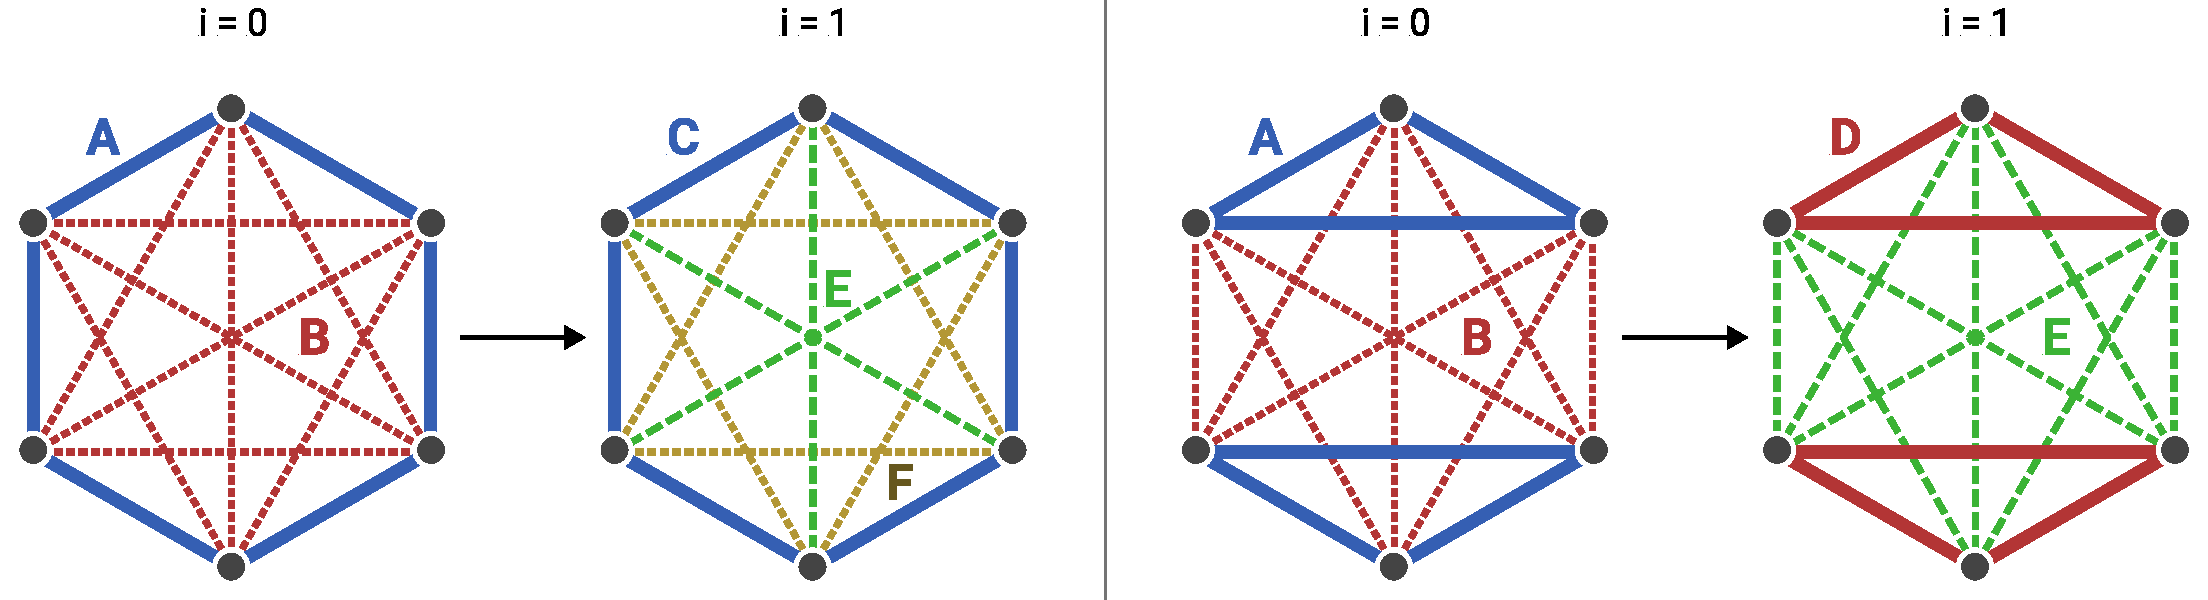
\includegraphics[width=\linewidth]{gfx/related-work/wl2-problem-solution.pdf}
	\caption{
		Two non-isomorphic graphs with $G \mathrel{\simeq_1} H$ and $G \mathrel{\not\simeq_2} H$.
	}\label{fig:related:wl2-problem-solution}
\end{figure}
\Cref{fig:related:wl2-problem-solution} illustrates \cref{cor:related:wl-monotonous} by showing how 2-WL is able to distinguish the two 1-WL indistinguishable graphs from \cref{fig:related:wl1-problem}.
Since the time complexity of $k$-\acs{wl} grows exponentially with $k$~\cite[cor.~1.9.7]{Immerman1990}, it does not provide an efficient universal solution to \ac{gi}.
However it turns out that almost all graphs are \ac{wl} distinguishable even for a small constant $k$.

For $k = 1$ \citet{Babai1980} have shown that two randomly selected non-isomorphic graphs $G \not\simeq H$ of size $n$ are 1-\acs{wl} indistinguishable with probability $n^{-\nicefrac{1}{7}}$.
Thus 1-\acs{wl} is already able to distinguish most graphs; it fails however to distinguish any pair of unlabeled $d$-regular graphs of the same size~\cite[cor.~1.8.5]{Immerman1990}.
\begin{defn}
	A graph $G$ is called \textit{$d$-regular} ($\mathit{rg}_d(G)$) iff.\ $\forall v \in \mathcal{V}_G: {|\Gamma_G(v)|} = d$.
\end{defn}
We have already seen this in \cref{fig:related:wl1-problem} since the ``six-cycle'' and the ``two-triangles'' graphs are in fact both 2-regular and of size 6.
This restriction alone is typically not an issue in the context of \ac{gcr} though, as molecular structures or social interaction graphs for example are rarely perfectly regular.
A more relevant restriction of 1-\acs{wl} is the fact that it is unable to detect cycles of length $m \geq 3$.
\begin{defn}\label{defn:related:wl-compute}
	$k$-\acs{wl} \textit{computes} a function $f: \mathcal{G} \to Y$ iff.\ that function can be expressed as $f(G) = g(\mathit{dist}_{\chi_{G, k}^{*}})$ via some function $g: (\mathcal{C} \to \mathbb{N}) \to Y$.
\end{defn}
\begin{defn}\label{defn:related:wl-count-detect}
	$k$-\acs{wl} \textit{counts} a certain subgraph $S$ iff.\ it computes $\mathit{count}_S(G) \coloneqq \left|\{ \hat{v}\, |\, v \in \mathcal{V}_G^{*} \land G[v] \equiv S \}\right|$ (see~\cref{defn:related:ordered-subgraph}).
	Similarly $k$-\acs{wl} \textit{detects} a subgraph $S$ iff.\ it computes $\mathit{contain}_S(G) \coloneqq \mathbbm{1}[\mathit{count}_S(G) > 0]$, with $\mathbbm{1}$ denoting the indicator function.
\end{defn}
To see why 1-\acs{wl} is unable to detect $m$-cycles in graphs, note that \cref{fig:related:wl1-problem} already contradicts the positive statement for $m = 3$;
this counterexample can be trivially generalized to all larger $m$ by replacing the ``six-cycle'' graph with a ``$(2m)$-cycle-graph'' graph and the ``two-triangles'' graph with a ``two-$m$-cycles'' graph which preserves the 2-regularity and therefore the 1-\acs{wl} indistinguishability.

This cycle-detection restriction of 1-\acs{wl} is relevant in practice because cycle counts are used in many domains to analyze graphs, e.g.\ triangle counts are commonly used in social network analysis to find interaction clusters~\cite{Milo2002}\cite{Newman2003}\cite{Welser2007} and the detection of 4-, 5- or 6-cycles is required to determine important chemical properties like the aromaticity of a molecule~\cite{Adamson1973}\cite{Kekule1866}.

If we increase the \acs{wl}-dimension to $k = 2$, the described 1-\acs{wl} restrictions no longer apply.
2-\acs{wl} is able to distinguish more than $1 - \mathcal{O}(\nicefrac{1}{n})$ of the regular $n$-vertex graphs~\cite[cor.~1.8.6]{Immerman1990} and can even count cycles:
\begin{prop}[see \citet{Fuerer2017} and \citet{Arvind2019} for the full proof]\label{prop:related:wl2-cycle-count}
	2-\acs{wl} is able to count $m$-cycles for $m \leq 7$ but it cannot detect 8-cycles.
\end{prop}
\begin{hproof}
	Only the idea behind triangle and 4-cycle counting is outlined here to give an intuition for why \cref{prop:related:wl2-cycle-count} holds.
	Note that the 2-\acs{wl} neighbors of each edge $(v, w) \in \mathcal{E}_G$ correspond to all possible paths $(v, u, w)$ of length 2, i.e.\ all possible triangles.
	By \cref{defn:related:wlk-refine} there must thus be a color subset $C^{\triangle}_j \subseteq \mathcal{C}$ representing that an edge is involved in exactly $j$ triangles after one refinement step.
	2-\acs{wl} then trivially counts triangles by setting $g(\mathit{dist}_\chi) = \frac{1}{3} \sum_j j \sum_{c \in C^{\triangle}_j} \mathit{dist}_\chi(c)$ to satisfy \cref{defn:related:wl-compute}.
	Analogously for 4-cycles, let $C^{\square}_j \subseteq \mathcal{C}$ be the colors indicating a non-edge $(v, w) \notin \mathcal{E}_G$ with $j$ common vertex neighbors $u \in \Gamma_G(v) \cap \Gamma_G(w)$.
	The number of 4-cycles is then determined by the colors of the diagonals through them via $g(\mathit{dist}_\chi) = \frac{1}{2} \sum_{j \geq 2} \binom{j}{2} \sum_{c \in C^{\square}_j} \mathit{dist}_\chi(c)$.
	Using a similar but more involved combinatorial argument requiring multiple color refinement steps, 5-, 6- \& 7-cycle counting can be shown.
\end{hproof}
As we just saw, 2-\acs{wl} is significantly more powerful than 1-\acs{wl}.
Though, by \cref{prop:related:wl-upper}, there are of course still 2-\acs{wl} indistinguishable graphs;
among others those are the strongly regular graphs $\mathit{srg}_{n, d, \lambda, \mu}(G)$.
\begin{defn}
	$\begin{aligned}[t]
		\mathit{srg}_{n, d, \lambda, \mu}(G) \iff\ & {|\mathcal{V}_G|} = n \quad\land\quad \forall v \in \mathcal{V}_G: {|\Gamma_G(v)|} = d \\
		&\land \forall (v, w) \in \mathcal{E}_G: {|\Gamma_G(v) \cap \Gamma_G(w)|} = \lambda \\
		&\land \forall (v, w) \in \mathcal{V}_G^2 \setminus \mathcal{E}_G: {|\Gamma_G(v) \cap \Gamma_G(w)|} = \mu
	\end{aligned}$
\end{defn}
Generally this restriction of 2-\acs{wl} is not an issue since strongly regular graphs do not appear in typical \ac{gcr} datasets.
By going to $k = 3$, even some strongly regular graphs as well as all planar graphs can be distinguished though~\cite{Kiefer2017}.
Apart from that there are currently few results regarding the classes of distinguishable graphs and computable functions for even higher \ac{wl}-dimensions.

\subsection{Spectral Graph Theory}%
\label{sec:related:character:spectral}

Let us now look at an alternative perspective on graph characterization which is provided by \textit{spectral graph theory}.
While \ac{wl} characterizes a graph via its color distribution $\mathit{dist}_{\chi_{G,k}^{*}}$, the spectral approach uses its so-called \textit{spectrum} $\lambda_G = (\lambda_{G, 1}, \dots, \lambda_{G, n}) \in \mathbb{R}^n$ where $n = |\mathcal{V}_G|$.
The key idea behind this is to interpret the adjacency matrix $A_G \in \mathbb{R}^{n \times n}$ of $G$ not simply as an encoding of the edges ($A_{G,i,j} = \mathbbm{1}[(v_i, v_j) \in \mathcal{E}_G]$) but as a linear operator $A_G: (\mathcal{V}_G \to \mathbb{R}) \to (\mathcal{V}_G \to \mathbb{R})$ acting on the vector space of real-valued functions with a vertex domain.
This means that $A_G$ transforms so-called \textit{graph signals} $x: \mathcal{V}_G \to \mathbb{R}$ which are functions assigning \textit{signal strengths} to vertices.
By applying $A_G x$ the signal strength $x[v_i]$ of each vertex is added to the signal strengths of its neighbors $\Gamma_G(v_i)$.
Using this functional perspective, one can characterize graphs via the \acf{ft}.
We will now see how this is done;
however, since a comprehensive description of spectral graph theory would exceed the scope of this thesis, only a brief overview will be given.
For a more detailed introduction to the field we refer to \citet{Shuman2013}.

\paragraph{The classical \acl{ft}}
Let us begin by describing the \ac{ft} for the more common case of functions with real domains.
All functions $f: \mathbb{R} \to \mathbb{R}$ can be interpreted as infinite-dimensional vectors $f = \int_{\mathbb{R}} f(t)\, b_t \dif t$ with $b_t: \mathbb{R} \to \mathbb{R}$ being a standard basis vector/function defined as $b_t(s) \coloneqq \begin{cases} 1 & \text{if } s = t \\[-6pt] 0 & \text{else} \end{cases}$. % chktex 21
The values of $f$ are then described as its $b_t$ components $\langle b_t, f \rangle = f(t)$, where $\langle b_t, \cdot \rangle = \delta_t(\cdot)$ denotes the Dirac delta function translated by $t$.
The \acl{ft} $\hat{f} = \mathcal{F}(f)$ of $f$ corresponds to a change of basis from the standard basis vectors $b_t$ to the Fourier basis vectors $u_\xi(t) \coloneqq e^{2 \pi i \xi t}$, i.e.\ $f = \int_{\mathbb{R}} \hat{f}(t)\, u_\xi \dif \xi$.
The Fourier basis is characterized by the fact that it is an eigenbasis of the so-called \textit{Laplace operator} $\Delta$, i.e.\ $\Delta u_\xi = \lambda_\xi u_\xi$ with $\lambda_\xi$ being the eigenvalue corresponding to $u_\xi$.
In the real domain this Laplace operator $\Delta$ is effectively the same as the second-derivative $\frac{\dif^2}{\dif t^2}$.
Thus it is easy to see that indeed $\Delta u_\xi = -\frac{\dif^2}{\dif t^2} u_\xi = \lambda_\xi u_\xi$ for $\lambda_\xi = {(2 \pi \xi)}^2$.

\paragraph{The graph \acl{ft}}
To extend the notion of the \ac{ft} from real functions $f: \mathbb{R} \to \mathbb{R}$ to graph signals $x: \mathcal{V}_G \to \mathbb{R}$ we need to define a graph variant of the Laplace operator $\Delta$.
It turns out that there are multiple possible ways to do so, the most simple being the so-called \textit{combinatorial graph Laplacian}.
\begin{defn}\label{defn:related:laplacian-comb}
	The combinatorial graph Laplacian $L_G \in \mathbb{R}^{n \times n}$ is defined as
	\begin{align*}
		L_G \coloneqq D_G - A_G\quad\text{with the degree matrix } D_G\coloneqq {
			\renewcommand*{\arraystretch}{0.5}
			\begin{pmatrix}
				d_1 & & \\
				& \ddots & \\
				& & d_n
			\end{pmatrix}
		}, d_i \coloneqq |\Gamma_G(v_i)| \text{.}
	\end{align*}
\end{defn}
Using this definition, applying $L_G x$ is analogous to taking the second derivative $\frac{\dif^2}{\dif t^2} f$.
Putting both Laplacian variants, $L_G$ and $\frac{\dif^2}{\dif t^2}$, side-by-side gives an intuition for why this is the case:
\begin{equation*}
	\begin{split}
		-\frac{\dif^2}{\dif t^2} f(t) = \smashoperator[l]{\lim_{h \to 0}} \frac{1}{h^2} (\underbrace{f(t) - f(t-h)}_{\Delta_{t, t-h}} + \underbrace{f(t) -  f(t+h)}_{\Delta_{t, t+h}})
	\end{split}
	\begin{split}\ \left|\ %
		L_G x[v] = \smashoperator[l]{\sum_{u \in \Gamma_G(v)}}\mkern-6mu \underbrace{(x[v] - x[u])}_{\Delta_{v, u}}
	\right.\end{split}
\end{equation*}
The second derivative of a function $f$ essentially averages the value differences in the neighborhood of a point $t$.
For real-valued functions this neighborhood only consists of the two infinitesimally close points to the left and to the right of $t$, i.e.\ $t - h$ and $t + h$.
The combinatorial graph Laplacian represents the same operation, where each point/vertex $v$ might however have more than two neighbors $u \in \Gamma_G(v)$ that need to be averaged.

The \ac{ft} of a graph signal $x$ then is $\hat{x}[i] = \langle u_{G,i}, x \rangle$ with $u_G = {\{ u_{G,i} \}}_{i=1}^{n}$ being the eigenvectors of $L_G$, s.t.\ $x = \sum_{i=1}^n \hat{x}[i] u_{G,i}$.
Since the set of Laplacian eigenvectors is finite, we can express the graph \ac{ft} $\mathcal{F}_G$ as a change of basis matrix $U_G = \begin{pmatrix} u_{G,1,1} & \cdots & u_{G,1,n} \\ \vdots & \ddots & \vdots \\ u_{G,n,1} & \cdots & u_{G,n,n} \end{pmatrix} \in \mathbb{R}^{n \times n}$.
Similarly the inverse \ac{ft} can be expressed as $\mathcal{F}^{-1} = U_G^{-1} = U_G^{\top}$ because $U_G$ is a real orthogonal matrix.
To see why this is the case, note that $L_G$ is guaranteed to only have real eigenvectors $u_G$ and eigenvalues $\lambda_G$ due to the fact that we only consider undirected graphs with symmetric adjacency matrices $A_G$.

\paragraph{Interpretation of the spectrum}
By convention we assume that the eigenvalues are ordered ascendingly: $\lambda_{G,0} \leq \cdots \leq \lambda_{G,n}$.
Those eigenvalues are called the \textit{spectrum of $G$} and they are a vertex-permutation-invariant graph characterization.
Intuitively those eigenvalues describe the connectivity between different parts of the graph.
The first eigenvalues represent connectivity at a general, coarse level while the last eigenvalues represent the connectivity of finer substructures.
\Cref{fig:related:graph-fourier} illustrates this idea.
A concrete example for the relation between a graph's structure and its spectrum is the fact that a graph with $m$ connected components has exactly $m$ zero eigenvalues, i.e.\ $0 = \lambda_{G,1} = \cdots = \lambda_{G,m} < \lambda_{G,m+1}$.
For a more detailed discussion of this relation we refer to \citet{Das2004}.
We will now instead look at the discriminative power of the spectrum.
\begin{figure}[ht]
	\centering
	\includegraphics[width=\linewidth]{gfx/related-work/graph-fourier.pdf}
	\caption[Comparison between the basis vectors of the real domain \acl{ft} and the graph \acl{ft}.]{
		Comparison between the basis functions/vectors of the real domain \ac{ft} and the graph \ac{ft}.
		For the eigenfunctions on the upper half only the real cosine components of the complex exponentials are shown.
		\source[based on]{Shuman2013}
	}\label{fig:related:graph-fourier}
\end{figure}
\begin{defn}\label{defn:related:cospectral}
	Two graphs $G$ and $H$ are \textit{cospectral} ($G \mathrel{\simeq_\lambda} H$) iff.\ $\forall i: \lambda_{G,i} = \lambda_{H,i}$.
\end{defn}

{\setlength{\parskip}{0pt}\paragraph{Spectral graph comparisons}
\citet{Alzaga2010} have shown that, while the cospectrality test can be more powerful than 1-\acs{wl}, it is always weaker than 2-\acs{wl}, i.e.\ $G \mathrel{\simeq_2} H \implies G \mathrel{\simeq_\lambda} H$.
Despite this limit on the discriminative power of the graph spectrum, it is still useful for determining graph similarity, e.g.\ by defining a distance measure on the vector space of spectra (see \citet{Gu2015}).}

As briefly mentioned before, the combinatorial graph Laplacian $L_G$ is not the only possible choice of graph Laplacian.
Note that the eigenvalues of $L_G$ grow with the number of edges\footnote{
	This is trivially shown by $\sum_{i=1}^n \lambda_{G,i} = \Tr(L_G) = \Tr(D_G) = |\mathcal{E}_G|$.
}.
Consequently a small graph $G$ will typically have a large spectral distance to a large graph $H$ (assuming ${|\mathcal{V}_G|} \ll {|\mathcal{V}_H|}$) irrespective of their similarity when ignoring the scale difference.
In domains where the absolute size of a graph should not influence its spectral characterization, it can therefore be useful to normalize the spectrum.
One common way to do so is via the so-called \textit{symmetric normalized Laplacian} $L^{\text{sym}}_G$.
\begin{defn}\label{defn:related:laplacian-sym}
	$L^{\text{sym}}_G \coloneqq D^{-\frac{1}{2}} L_G D^{-\frac{1}{2}}$ is the symmetric normalized Laplacian of $G$.
\end{defn}
The eigenvalues $\lambda^{\text{sym}}_{G, i}$  of this Laplacian all lie in the range $[0, 2]$.
\Cref{fig:related:spectral-normalization} illustrates how this makes it possible to compare the structure of graphs across varying vertex counts.
Besides $L^{\text{sym}}_G$ there are also other ways to normalize the spectrum, e.g.\ by using the random walk Laplacian $L^{\text{rw}}_G \coloneqq D^{-1} L_G$, which will however not be covered here (see \citet{Shuman2013}).
\begin{figure}[ht]
	\centering
	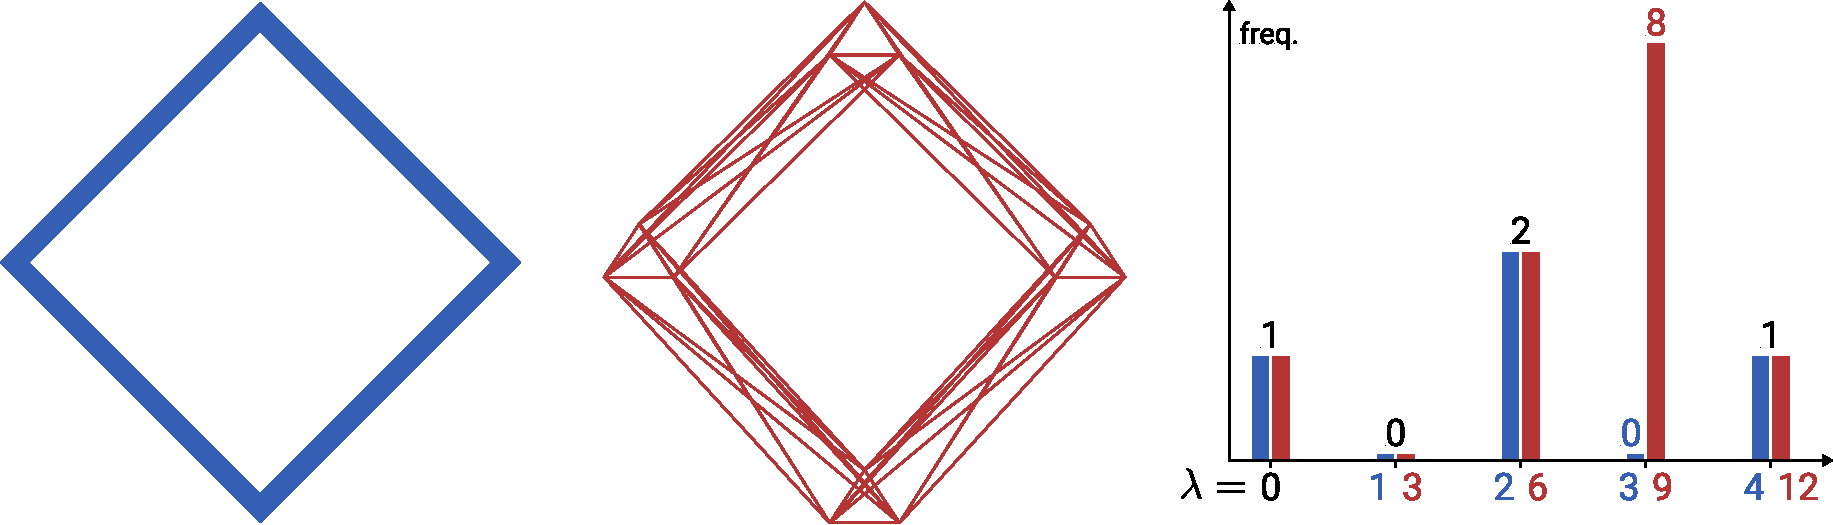
\includegraphics[width=\linewidth]{gfx/related-work/spectral-normalization.pdf}
	\caption[Comparison of the unnormalized $L_G$ spectrum and the normalized $L^{\text{sym}}_G$ spectrum.]{
		Comparison of the unnormalized $L_G$ spectrum and the normalized $L^{\text{sym}}_G$ spectrum.
		Two structurally similar graphs of different size are compared.
		The \textcolor{t_red}{large graph} is derived by replacing each vertex of the \textcolor{t_blue}{small 4-cycle graph} by a triangle.
		While their unnormalized spectra have different absolute ranges (\textcolor{t_blue}{$[0, 4]$} vs.\ \textcolor{t_red}{$[0, 12]$}), the histogram on the right shows that their normalized eigenvalue distributions align.
	}\label{fig:related:spectral-normalization}
\end{figure}

\section{Graph Classification and Regression}%
\label{sec:related:gcr}

The existing approaches to tackle the \ac{gcr} problem can be categorized into three main families:
\begin{enumerate*}
	\item Explicit graph embeddings,
	\item graph kernels and
	\item graph neural networks
\end{enumerate*}.
We will now look at the characteristics of those families and give a brief overview of specific methods.

\subsection{Explicit Graph Embeddings}%
\label{sec:related:gcr:embed}

The basic idea of explicit graph embedding approaches is to map a graph $G \in \mathcal{G}$ to some vector in a finite vector space $\mathcal{X} = \mathbb{R}^d$.
A function $\varphi: \mathcal{G} \to \mathcal{X}$ is called a \textit{graph embedding function}.
By embedding a graph into $\mathcal{X}$, any classification or regression algorithm that works with vectors can then be applied to solve the \ac{gcr} problem.

The so-called vertex embedding problem is closely related to the graph embedding problem.
As the name suggests, a \textit{vertex embedding function} $\varphi_G$ maps all vertices $v \in \mathcal{V}_G$ to $\mathcal{X}$.
The embedding vector $\varphi_G(v)$ ideally encodes relevant information about a vertex and its structural position in $G$.
It can be used to solve the vertex classification and regression problem via arbitrary \ac{ml} methods for vectors.
We will now look at two main families of explicit graph and vertex embedding approaches.

\subsubsection{Fingerprint Embeddings}

The first works on graph embeddings were motivated by the study of chemical structures~\cite{Adamson1973}\cite{Willett1986}.
There a molecule can be interpreted as a labeled graph for which the \ac{gcr} problem corresponds to the prediction of some chemical property, e.g.\ toxicity or solubility.
So-called \textit{fingerprint embeddings} try to match a fixed set of subgraphs $S_1, \dots, S_d$ to the input graph.
The embedding of a graph $G$ is a binary vector $\varphi(G) = x \in {\{0, 1\}}^d$ with $x_i \coloneqq \mathit{contain}_{S_i}(G)$ (see~\cref{defn:related:wl-count-detect}).
This simple approach usually requires a careful choice of subgraphs but can still be competitive with the other more recent approaches we will look at in the following sections.
Fingerprint embeddings are for example used in multiple state-of-the-art toxicity prediction tools like RASAR~\cite{Luechtefeld2018}\cite{ToxTrack}, ProTox~\cite{Drwal2014}\cite{ProTox}\cite{Banerjee2018} or the \ac{toxTest}~\cite{TEST}.

\subsubsection{Skip-gram inspired Embeddings}

Skip-gram embeddings were introduced by \citeauthor{Mikolov2013} as part of the well-known \texttt{word2vec}~\cite{Mikolov2013} word embedding method from \ac{nlp}.
While a fingerprint embedding explicitly assigns an interpretation to each embedding dimension (i.e.\ to each standard basis vector), a skip-gram embedding only optimizes the distance between embedding vectors based on the similarity of the embedded instances without providing an interpretation of the embedding dimensions.

\paragraph{word2vec}
Let us first look at the \texttt{word2vec} skip-gram method.
It gets a sequence of words $(w_0, \dots, w_n)$ as input and outputs embedding vectors $\varphi(w_0), \dots, \varphi(w_n) \in \mathbb{R}^d$.
To do this the context $\Gamma_k(w_i) = \{ w_{i-k}, \dots, w_{i + k} \}$ is computed for all words where $w_i$ is the so-called \textit{context root}.
The word contexts are then used to optimize the following log-likelihood objective:
\begin{gather}
	\max_{\varphi, \varphi_{\Gamma}} \sum_{i = 1}^n \log P(\Gamma_k(w_i) | w_i)\ =\ \max_{\varphi, \varphi_{\Gamma}} \sum_{i = 1}^n \smashoperator[r]{\sum_{w_j \in \Gamma_k(w_i)}}\, \left[ {\varphi(w_i)}^\top \varphi_{\Gamma}(w_j) - \log Z_{w_i} \right] \label{eq:related:word2vec}\\
	\text{with } P(\Gamma_k(w_i) | w_i) \coloneqq \prod_{\mathclap{w_j \in \Gamma_k(w_i)}}\, \overbrace{\frac{\exp\left({\varphi(w_i)}^\top \varphi_{\Gamma}(w_j)\right)}{Z_{w_i}}}^{P(w_j | w_i)}
	\text{ and } Z_{w_i} \coloneqq \sum_{j = 1}^n \exp\left({\varphi(w_i)}^\top \varphi_{\Gamma}(w_j)\right) \nonumber
\end{gather}
\texttt{word2vec} essentially uses an expectation maximization scheme to maximize the probabilities $P(w_j | w_i)$ of observing the context words $w_j \in \Gamma_k(w_i)$ of all words $w_i$.
Those probabilities are described by the overlap of the embeddings $\varphi(w_i)$ of words $w_i$ and the embeddings $\varphi_{\Gamma}(w_j)$ of their context words $w_j$.
Intuitively this means that words with similar contexts will be mapped close to each other in the embedding space.
Note that \texttt{word2vec} actually finds two embeddings $\varphi(w)$ and $\varphi_{\Gamma}(w)$ for each word of which only the first is returned.
The two embeddings represent two different perspectives on words: $\varphi$ describes a word $w_i$ as the root of a context $\Gamma_k(w_i)$, $\varphi_{\Gamma}$ on the other hand describes a word $w_j$ as part of a context $\Gamma_k(w_i) \ni w_j$.

\paragraph{Vertex Embeddings}
Skip-gram embeddings can be  na{\"\i}vely extended to graphs by realizing that \texttt{word2vec} effectively already is a vertex embedding method for linear graphs in which $\Gamma_k(v)$ is simply the $k$-neighborhood of the vertex/word $v$.
The problem with this na{\"\i}ve extension is that the sizes of $k$-neighborhoods in arbitrary graphs can be much larger and often tend to grow exponentially with $k$.
To deal with this computational problem the so-called DeepWalk~\cite{Perozzi2014} and \texttt{node2vec}~\cite{Grover2016} methods perform random walks of fixed length to effectively take samples from the neighborhood of vertices.
Both methods only differ in the transition matrix that is used for the random walk.
Another difference of DeepWalk and \texttt{node2vec} compared to \texttt{word2vec} is the so-called \textit{feature space symmetry} which states that the context root interpretation ($\varphi$) of a vertex should be symmetric to its context element interpretation ($\varphi_{\Gamma}$), i.e.\ $\varphi = \varphi_{\Gamma}$.
The combination of random walk context sampling and and the feature space symmetry assumption can be used to compute vertex embeddings even for very large graphs.

\paragraph{Graph Embeddings}
Skip-gram methods can not only be used for vertex embeddings but also to embed entire graphs.
One way to do this is via the \texttt{graph2vec}~\cite{Narayanan2017} method.
It is inspired by \texttt{doc2vec}~\cite{Le2014} which in turn is based on \texttt{word2vec}.
\texttt{graph2vec} gets a set of graphs $\mathcal{G} = \{ G_1, \dots G_N \}$ as input and outputs graph embeddings $\varphi(G_1), \dots, \varphi(G_N)$.
While in \texttt{word2vec} every word can be a context root as well as a context element, \texttt{graph2vec} uses the graphs $\mathcal{G}$ as context roots.
The context $\Gamma_T(G_i)$ of a graph $G_i$ is defined as
\begin{equation}
	\Gamma_T(G_i) \coloneqq \bigcup_{\mathclap{v_j \in \mathcal{V}_{G_i}}}\, {\left\{ \chi_{G_i, 1}^{(t)}(v_j) \right\}}_{t = 0}^T % chktex 21
	\quad\text{with $T \in \mathbb{N}$ and $\chi_{G_i, 1}^{(t)}$ as in \cref{defn:related:wl1-refine}.}
\end{equation}
Intuitively this context can be understood as the set of 1-\acs{wl}-distinguishable subgraphs of $G_i$ with diameter $\leq 2T$.
Since \ac{wl} is used to identify distinct subgraphs, \texttt{graph2vec} can only be applied to graphs with discrete vertex labels.
Using the previous definitions, the context root embedding function has the signature $\varphi: \mathcal{G} \to \mathbb{R}^d$ while the context element embedding function is of type $\varphi_{\Gamma}: \bigcup_{G_i \in \mathcal{G}} \Gamma_T(G_i) \to \mathbb{R}^d$.
To find those embeddings the \texttt{word2vec} objective from \cref{eq:related:word2vec} is reused.
Analogous to \texttt{word2vec}, \texttt{graph2vec} therefore embeds graphs that share subgraphs close to each other, whereas graphs that do not share substructures tend to be embedded further away from each other.

\subsection{Graph Kernels}%
\label{sec:related:gcr:kernel}

Instead of mapping a graph into an explicitly defined vector space of fixed dimension, one can also do so implicitly by employing the kernel trick.
There is a large variety of so-called \acp{gk} to do this.
\acp{gk} can be used in combination with any kernelized learner, typically \acp{svm}, to solve the \ac{gcr} problem.
While there is a large variety of different \acp{gk}~\cite{Kriege2020}, we will focus on those that are based on the previously described family of \ac{wl} algorithms.

\paragraph{\ac{wl} subtree kernel}
One well-known \ac{gk} is based directly on the 1-\acs{wl} coloring algorithm, the so-called \textit{\ac{wl} subtree kernel}~\cite{Shervashidze2011}.
It is uses the mapping
\begin{align}
	\varphi_{\text{ST}}(G) \coloneqq \bigoplus_{t=0}^{T} {\left( \mathit{dist}_{\chi_{G,1}^{(t)}}(c) \right)}_{c \in \mathcal{C}}
	\quad\text{with $\oplus$ denoting vector concatenation.} \label{eq:related:wl-subtree-kernel}
\end{align}
$\varphi_{\text{ST}}(G)$ encodes the color counts across a fixed number $T$ of 1-\acs{wl} refinement steps.
Via this mapping, the \ac{wl} subtree kernel function $k_{\text{ST}}: \mathcal{G} \times \mathcal{G} \to \mathbb{R}$ can then be simply written as the standard inner vector product $k_{\text{ST}}(G, H) \coloneqq \langle \varphi_{\text{ST}}(G), \varphi_{\text{ST}}(H) \rangle$.
\begin{figure}[ht]
	\centering
	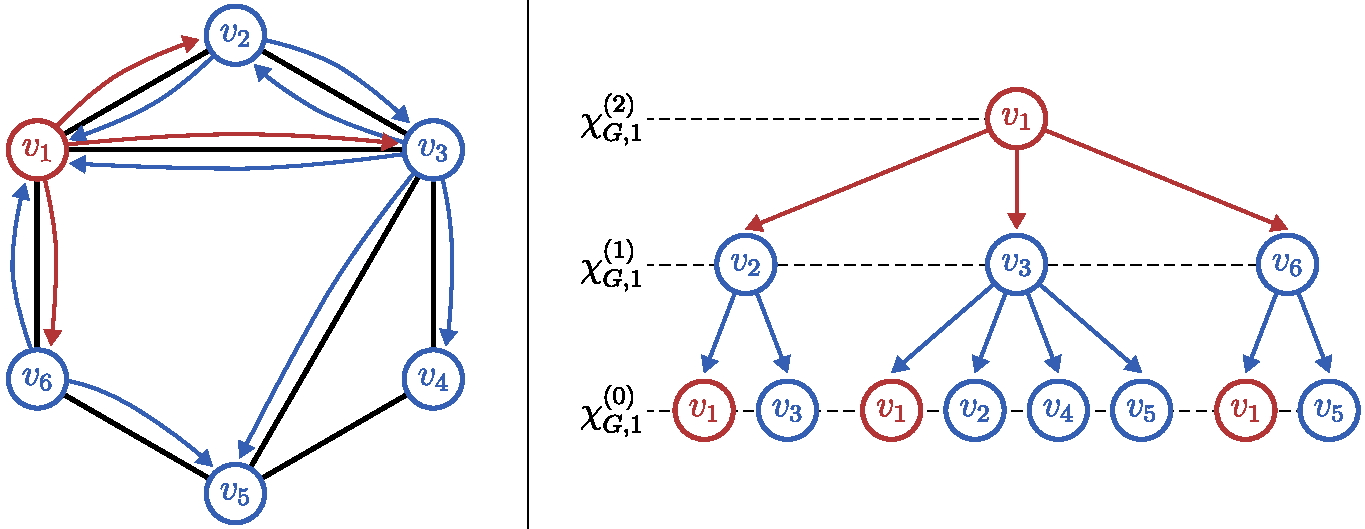
\includegraphics[width=0.7\linewidth]{gfx/related-work/wl-subtree.pdf}
	\caption[Illustration of the correspondence between the \ac{wl} color $\chi_{G,1}^{(t)}(v)$ and the breadth-first subtree of depth $l$ rooted at $v$.]{
		Illustration of the correspondence between the \ac{wl} color $\chi_{G,1}^{(t)}(v)$ and the breadth-first subtree of depth $t$ rooted at $v$ (for $t = 2$ and $v = \texttt{\textcolor{t_blue}{\circled{1}}}$). % chktex 25
		\source[based~on]{Shervashidze2011}
	}\label{fig:related:wl-subtree}
\end{figure}

\Cref{fig:related:wl-subtree} illustrates how this definition relates to subtrees.
Since alls vertex colors $c \in \mathcal{C}$ correspond to a subtree isomorphism class, $k_{\text{ST}}(G, H)$ effectively computes the similarity of $G$ and $H$ by comparing their local subtree structures of depth at most $T$.
Note that the underlying mapping $\varphi_{\text{ST}}$ cannot be computed independently for each graph $G \in \mathcal{G}_{\mathcal{D}} \subseteq \mathcal{G}$ in a given training dataset $\mathcal{D}$ since the set of colors $c \in \mathcal{C}$ introduced by the hashing function $h$ is conjointly determined by all graphs $\mathcal{G}_{\mathcal{D}}$ (see \cref{defn:related:wl1-refine}).
Consequently the dimensionality $d$ of $\varphi_{\text{ST}}(G) \in \mathbb{N}^d$ varies, depending on the entire dataset $\mathcal{D}$.

\paragraph{\ac{wl} shortest path kernel}
Extending the idea of the \ac{wl} subtree kernel, the \textit{\ac{wl} shortest path kernel}~\cite{Shervashidze2011}\cite{Borgwardt2005} adds global structural information to the local subtree comparisons.
The $i$-th component of a graph's shortest path vector $\varphi_{\text{SP}}(G)$ corresponds to the 4-tuple $(t_i, a_i, b_i, d_i) \in {\{ 0, \dots, T \}} \times \mathcal{C} \times \mathcal{C} \times \mathbb{N}$ and its value is described by
\begin{align}
	{\varphi_{\text{SP}}(G)}_i \coloneqq \left| \left\{ (v, u) \in \mathcal{V}_G^2 \,|\, {\chi_{G,1}^{(t_i)}(v) = a_i} \land {\chi_{G,1}^{(t_i)}(u) = b_i} \land {d_{\text{SP}}(v, u) = d_i} \right\} \right| \text{,} % chktex 21
\end{align}
with $d_{\text{SP}}(v, u)$ denoting the length of the shortest path from $v$ to $u$ in $G$.
Analogous to $k_{\text{ST}}$, the shortest path kernel function is defined as $k_{\text{SP}}(G, H) \coloneqq \langle \varphi_{\text{SP}}(G), \varphi_{\text{SP}}(H) \rangle$.
Since $\varphi_{\text{SP}}(G)$ has one component for each possible 4-tuple $(t_i, a_i, b_i, d_i)$, its dimensionality grows quadratically with the total number of introduced 1-\acs{wl} colors $\mathcal{C}$ and linearly with the length of the longest shortest path $\max_{G \in \mathcal{G}_{\mathcal{D}}, (v, u) \in \mathcal{V}_G^2} d_{\text{SP}}(v, u)$.
While this approach is computationally significantly more expensive than the subtree kernel, it also has a higher discriminative power and allows the shortest path kernel to distinguish even some 1-\acs{wl} indistinguishable graphs.
The subtree kernel only compares graphs by the presence of local subtrees;
the shortest path kernel additionally checks how well the distances between those subtrees align.
Looking back at the 1-\acs{wl} indistinguishable ``six-cycle''/``two-triangles'' example from \cref{fig:related:wl1-problem}, we see that this additional information distinguishes the two graphs due to the fact that the longest shortest path in a six-cycle has length 3 while the longest shortest path in a triangle is of length 1.

\paragraph{Higher dimensional \ac{wl} kernels}
Instead of incorporating shortest path information to increase the power of the \ac{wl} kernel, one can alternatively just increase the \acs{wl}-dimension $k$.
A na{\"\i}ve generalization of the 1-\acs{wl} subtree kernel would simply use \cref{eq:related:wl-subtree-kernel} but with the k-\acs{wl} colorings $\chi_{G,k}^{(t)}$ instead of $\chi_{G,1}^{(t)}$.
The problem with this approach is that the runtime of \ac{wl} increases exponentially with $k$;
even for $k = 2$ the cost often becomes infeasibly high when working with large graphs.
To tackle this problem \citet{Morris2017} proposed a combination of two optimizations:
\begin{enumerate}[label=\textbf{\arabic*.}]
	\item \textbf{$k$-multisets:}
		The first optimization is to assign colors to vertex $k$-multisets instead of vertex $k$-tuples, where a $k$-multiset is any multiset $s \subseteq \mathcal{V}_G$ with ${|s|} = k$.
		This reduces the amount of colors that have to be refined in each \ac{wl} iteration by a factor of $k!$. % chktex 40
		Based on \cref{defn:related:wlk-refine}, the multiset color refinement step is defined as
		\begin{align}
			\chi_{G,k}^{(t+1)}(s) \coloneqq h\left(\chi_{G,k}^{(t)}(s), \ldblbrace \{ \chi_{G,k}^{(t)}(s \setminus \{v\} \cup \{u\})\, |\, v \in s \}\, |\, u \in \mathcal{V}_G \rdblbrace\right) \text{.} \label{eq:related:wlk-set-refine} % chktex 21
		\end{align}
		Even though this simplification generally reduces the discriminative power of the kernel, for $k = 2$ specifically no information and therefore no power is lost by replacing the tuples $(v, u)$ and $(u, v)$ with $\ldblbrace v, u \rdblbrace$ since the undirectedness of graphs implies that $\chi_{G,2}^{(t)}(v, u) = \chi_{G,2}^{(t)}(u, v)$ even when doing tuple-based color refinement.
	\item \textbf{Neighborhood localization:}
		The second optimization uses the fact that most real-world graphs tend to be sparse~\cite{Chung2010}, i.e.\ ${|\mathcal{E}_G|} = \mathcal{O}(|\mathcal{V}_G|)$.
		The multiset-based $k$-\acs{wl} algorithm refines the color of a $k$-multiset $s$ by hashing the colors of its neighbors as defined in \cref{eq:related:wlk-set-refine} where there is one neighbor per vertex $u \in \mathcal{V}_G$.
		By the sparsity assumption, most of those vertices $u$ are however not connected with any of the vertices in $s$, i.e.\ $u \notin \Gamma_G(s)$ with $\Gamma_G(s) \coloneqq \bigcup_{v \in s} \Gamma_G(v)$.
		The refinement runtime can therefore often be reduced significantly by only considering ``local'' neighbors $u \in \Gamma_G(s)$ instead of the ``global'' neighborhood $u \in \mathcal{V}_G$ in \cref{eq:related:wlk-set-refine}.
\end{enumerate}
We call the kernel that only uses the first optimization \textit{$k$-GWL}~($k$-dim.\ global \ac{wl}) and the kernel that uses both optimizations \textit{$k$-LWL}~($k$-dim.\ local \ac{wl}).
\citet{Morris2017} have empirically shown that focusing on local graph structures via LWL often actually performs better than the computationally more expensive GWL kernel.

\subsection{Graph Neural Networks}%
\label{sec:related:gcr:nn}

The last family of \ac{gcr} approaches we will look at is that of \acp{gnn}.
The idea to feed a graph into a \ac{nn} was first described by \citet{Gori2005}.
Since then many variants and extensions of that idea have been proposed~\cite{Wu2019}.
We will focus specifically on the so-called \acp{gcnn} which can be divided into two variants:
Spectral and spatial \acp{gcnn}.

\subsubsection{Spectral \acp{gcnn}}

The class of spectral \acp{gcnn} is motivated by spectral graph theory (see \cref{sec:related:character:spectral}).
A spectral \ac{gcnn} expects a graph $G$ with real vertex feature vectors $x_G[v_i] \in \mathbb{R}^d$ as its input.
Those feature vectors are typically one-hot encodings of labels or, if no such information is provided, vertex embedding vectors (see \cref{sec:related:gcr:embed}).
We call $X_G \coloneqq \begin{pmatrix} x_G[v_1] \\ \vdots \\ x_G[v_n] \end{pmatrix} \in \mathbb{R}^{n \times d}$ the vertex feature matrix of $G$.
Note that each of the $d$ columns of $X_G$ can be interpreted as a separate graph signal function $x_{G,j}: \mathcal{V}_G \to \mathbb{R}$ for $j \in [d]$.
The core idea of spectral \acp{gcnn} is to learn a graph convolution kernel $g$, similar to the grid kernels in conventional \acp{cnn}~\cite{LeCun1998}.
The problem with this idea is that the convolution operation $g * x$ requires some notion of distance in order to ``move'' the kernel $g$ over the function $x$.
Graphs do not generally satisfy this requirement, i.e.\ the notion of a vertex distance $\|v_i - v_j\|$ is not clearly defined.
Via the convolution theorem $g * x = \mathcal{F}^{-1}(\hat{g} \odot \hat{x})$ we can however still define a graph convolution operator that works directly in the spectral domain:
\begin{align}
	g * x_{G,j} \coloneqq U_G^{\top} (\hat{g} \odot (U_G x_{G,j}))
	\text{ with $\odot$ denoting element-wise multiplication.} \label{eq:related:graph-conv-general}
\end{align}
To see the connection to the convolution theorem, remember that the Laplacian eigenvector matrices $U_G$ and $U_G^{\top}$ correspond to the \ac{ft} $\mathcal{F}$ and inverse \ac{ft} $\mathcal{F}^{-1}$ respectively.
In this formulation of convolution the Fourier transformed kernel $\hat{g}$ can be interpreted as a spectral filter, i.e.\ it dampens or amplifies certain eigenvector components of a graph.
\citet{Bruna2013}\cite{Henaff2015} first described a \ac{gnn} architecture that learns such a spectral filter $\hat{g}$.
Since a \ac{gnn} has to accept many different graphs of varying size $n$, the filter can however not be learned as a direct mapping $\hat{g}: [n] \to \mathbb{R}$.
Therefore it is not expressed in terms of the indices $i$ of specific eigenvectors $u_{G,i}$ but instead in terms of the corresponding eigenvalues\footnote{
	Here either the unnormalized eigenvalues of $L_G$ or the eigenvalues of some normalized Laplacian, e.g.\ $L_G^{\text{sym}}$, can be used.
} via $\hat{g}(\Lambda_G) = \begin{pmatrix} \hat{g}(\lambda_{G,1}) & & \\ & \ddots & \\ & & \hat{g}(\lambda_{G,n}) \end{pmatrix}$.
In order to learn such an eigenvalue filter $\hat{g}: \mathbb{R} \to \mathbb{R}$ via gradient descent, it requires some differentiable parameterization.

\paragraph{Chebyshev filters}
One such parameterization is based on the family of recursively defined Chebyshev polynomials $T_k(x) = 2x T_{k-1}(x) - T_{k-2}(x)$ with $T_0 = 1$ and $T_1 = x$~\cite{Defferrard2016}.
It describes a spectral filter as a linear combination $\hat{g}_{\theta}(\lambda) \coloneqq \sum_{k=0}^{K-1} \theta_k T_k(\lambda)$ with $\theta \in \mathbb{R}^K$.
This restricts $\hat{g}_{\theta}$ to be a polynomial which allows us to rewrite the graph convolution from \cref{eq:related:graph-conv-general} as
\begin{align}
	g_{\theta} * x_{G,j}
	\enspace=\enspace U_G^{\top}\, \hat{g}_{\theta}(\tfrac{2}{\max{\lambda_{G}}} \Lambda_G - I)\, U_G\, x_{G,j}
	\enspace=\enspace \hat{g}_{\theta}(\tfrac{2}{\max{\lambda_{G}}} L_G - I)\, x_{G,j} \label{eq:related:graph-conv-cheby} % chktex 21
\end{align}
because $L_G = U_G^{\top} \Lambda_G U_G$ is an eigendecomposition of the Laplacian.
The $\tfrac{2}{\max \lambda_{G}} \Lambda_G - I$ term normalizes the eigenvalues to $[-1, 1]$ which prevents vanishing and exploding gradients.
The advantage of this formulation is that it can be evaluated without actually having to compute the expensive eigendecomposition of $L_G$.
Instead, by interpreting $\hat{g}_{\theta}$ as a matrix polynomial, one only has to compute the powers $L_G^1, \dots, L_G^{K-1}$ and the largest eigenvalue $\max{\lambda_G}$ which is generally much cheaper than computing the full spectrum.

\paragraph{Linear filters}
\citet{Kipf2017} simplify the Chebyshev filter from \cref{eq:related:graph-conv-cheby} even further in the ambiguously named \ac{gcn} architecture\footnote{
	We use ``\acs{gcn}'' to refer to their proposed specific method in order to be consistent with other literature.
	We use ``\acs{gcnn}'' to refer to the broader family of \acl{gcnn} methods.
}.
By fixing $K = 2$, by using a single filter parameter $\theta \in \mathbb{R}$ and by assuming that $\max{\lambda_G^{\text{sym}}} \approx 2$ (see \cfullref{defn:related:laplacian-sym}) the convolution operation is reduced to
\begin{align}
	g_{\theta} * x_{G,j} = \theta \left( \tilde{D}_G^{-\frac{1}{2}} \tilde{A}_G \tilde{D}_G^{-\frac{1}{2}} \right) x_{G,j}
	\quad\text{with $\tilde{A}_G = A_G + I$ and $\tilde{D}_G = D_G + I$.} \label{eq:related:graph-conv-gcn}
\end{align}
In this formulation the spectral filter is effectively just a linear function $\hat{g}_{\theta}(\lambda) = \theta \lambda$.
Via this simplified notion of convolution for a single feature signal $x_{G,j}$, a convolutional \acl{nn} layer over all features ${\{ x_{G,j} \}}_{j=1}^{d}$ can analogously be defined as
\begin{align}
	Z^{(t)} \coloneqq \sigma\left( \hat{A} Z^{(t-1)} \Theta^{(t)} \right)
	\quad\text{with } \hat{A} \coloneqq \tilde{D}_G^{-\frac{1}{2}} \tilde{A}_G \tilde{D}_G^{-\frac{1}{2}}\quad\text{and}\quad Z^{(0)} \coloneqq X_G \text{.} \label{eq:related:gcn-layer}
\end{align}
Here $\sigma$ is some non-linearity, e.g.\ ReLU, and $\Theta^{(t)} \in \mathbb{R}^{d^{(t-1)} \times d^{(t)}}$ is a matrix of learned filter parameters.
This type of convolutional layer takes a graph signal $Z^{(t-1)} \in \mathbb{R}^{n \times d^{(t-1)}}$ and the corresponding adjacency matrix $A_G \in \mathbb{R}^{n \times n}$ as input and outputs a convolved signal $Z^{(t)} \in \mathbb{R}^{n \times d^{(t)}}$.
By stacking multiple of those convolutional layers, complex non-linear signal filters can be learned despite the linearity of the underlying spectral filter.

\subsubsection{Spatial \acp{gcnn}}
Looking at the \ac{gcn} layer defined in \cref{eq:related:gcn-layer}, notice that, even though it is motivated by spectral graph theory, the spectrum $\lambda_G$ is not actually directly used.
This allows for a very different perspective on \acp{gcn}:
Instead of interpreting convolutions as applications of linear spectral filters, we can interpret them as vertex neighborhood aggregations, similar to 1-\acs{wl}.
From this perspective a \ac{gcn} can be seen as a so-called spatial \ac{gcnn} because it operates directly in the vertex domain.
To see why this is the case, we rewrite \cref{eq:related:gcn-layer} and compare it with the 1-\acs{wl} color refinement strategy (see \cfullref{defn:related:wl1-refine}):
\begin{align*}
	\text{\ac*{gcn}:}\quad&& Z^{(t)}[v] &= \sigma\left(\left( {c(v)}^2 Z^{(t-1)}[v] + \smashoperator[lr]{\sum_{u \in \Gamma_G(v)}} c(v) c(u) Z^{(t-1)}[u] \right) \Theta^{(t)} \right) \\
	\text{1-\acs{wl}:}\quad&& \chi_{G,1}^{(t)}(v) &= h\left( \chi_{G,1}^{(t-1)}(v), \ldblbrace \chi_{G,1}^{(t-1)}(u)\, |\, u \in \Gamma_{G}(v) \rdblbrace\right)
\end{align*}
Here $c(v) \coloneqq {\left(\left| \Gamma_G(v) \right| + 1\right)}^{-\frac{1}{2}}$ are normalization factors introduced by $\tilde{D}_G^{-\frac{1}{2}}$.
The comparison shows that \ac{gcn} convolutions can be understood as iterative refinements of continuous ``color vectors'' $Z^{(t)}[v] \in \mathbb{R}^{d^{(t)}}$.
Then the continuous analogue to the injective 1-\acs{wl} hash function $h: \mathcal{C}^{*} \to \mathcal{C}$ can be defined as $h_{\text{\acs*{gcn}}}(z_0, z_1, \dots, z_m) = \sigma(\sum_{j=0}^m c(v_0) c(v_j) z_j \Theta^{(t)})$ which computes a single color vector from multiple color vectors $z_j$.

\paragraph{A 1-\acs{wl} bound on \ac{gnn} power}
The relation between \acp{gcnn} using neighborhood aggregation convolution and 1-\acs{wl} was formally analyzed by \citet{Xu2018}.
They show that the discriminative power of such a \ac{gcnn} is upper-bounded by that of 1-\acs{wl}.
In particular the \ac{gcn} architecture is strictly less powerful than 1-\acs{wl} due to the fact that $h_{\text{\acs*{gcn}}}$ is not an injective hash function.
To overcome this limitation an alternative neighborhood aggregation architecture called \ac{gin} was proposed:
\begin{align}
	Z^{(t)}[v] \coloneqq \text{\acs*{mlp}}^{(t)}\left( Z^{(t-1)}[v] + \smashoperator[lr]{\sum_{u \in \Gamma_G(v)}} Z^{(t-1)}[u] \right)
\end{align}
By leaving out the normalization factors $c(v)$ and by using a \ac{mlp} instead of the single fully-connected layer $\sigma \circ \Theta^{(t)}$ the resulting hashing function $h_{\text{\acs*{gin}}}(z_1, \dots, z_m) = \text{\acs*{mlp}}^{(t)}(\sum_{j=1}^{m} z_j)$ becomes injective\footnote{
	Under the assumption that the set of possible input feature matrices $X \in \mathbb{R}^{n \times d^{(0)}}$ is countable.
	This is reasonable since real-world \ac{gcr} domains typically only have a finite set of possible vertex feature vectors, e.g\ one-hot label encodings.
}, i.e.\ it assigns a unique color vector to each multiset of color vectors.
It was shown that this implies that \ac{gin} has the same discriminative power as 1-\ac{wl}.
As expected, \ac{gin} therefore fits training data better than non-injective \acp{gcnn} like \ac{gcn}.
Interestingly \ac{gin} additionally seems to generalize better on test data than non-injective methods~\cite{Xu2018}\cite{Errica2020}.
It is not yet fully understood why this is the case.

\paragraph{Higher dimensional \ac{wl} \acp{gnn}}
The majority of \ac{gnn} methods uses a neighborhood aggregation scheme which limits their discriminative and, more importantly, computational power to that of 1-\acs{wl} (see \cfullref{defn:related:wl-count-detect}).
To go beyond the limits of 1-\acs{wl}, \citet{Morris2019} proposed the first \ac{gcnn} architecture inspired by the higher dimensional $k$-\acs{wl} algorithms.
Similar to the $k$-LWL kernel which we looked at in \cref{sec:related:gcr:kernel}, their so-called $k$-\acs{gnn} uses the $k$-multiset and neighborhood localization optimizations to keep runtime costs feasible.
The $k$-\ac{gnn} convolution is described by
\begin{align}
	Z^{(t)}[s] \coloneqq \sigma\left( {Z^{(t-1)}[s]} W^{(t)} + \smashoperator[lr]{\sum_{v \in s, u \in \Gamma_G(v)}} {Z^{(t-1)}[s \setminus \{ v \} \cup \{ u \}]} W_{\Gamma}^{(t)} \right) \text{.} \label{eq:related:kgnn-layer}
\end{align}
It convolves the feature vectors of $k$-multisets $s \subseteq \mathcal{V}_G$ instead of single vertices $v \in \mathcal{V}_G$.
Apart from this fundamental difference to 1-\acs{wl} bounded \acp{gnn}, $k$-\acp{gnn} additionally use two learnable parameter matrices $W^{(t)}, W_{\Gamma}^{(t)} \in \mathbb{R}^{d^{(t-1)} \times d^{(t)}}$ instead of the single $\Theta^{(t)}$ used in \acp{gcn}.
This separation of the parameter matrix effectively fulfills the same purpose as the \ac{mlp} in \ac{gin}; it makes the implicitly defined $k$-\acs{gnn} hash function injective.
This can be seen by realizing that a stack of $k$-\acs{gnn} convolution layers with $W_{\Gamma}^{(t)} = 0$ for all but the first layer simulates a \ac{mlp}.

As a final remark, note that the concept of ``neighborhood'' in \cref{eq:related:kgnn-layer} is slightly different from that used by the $k$-\acs{wl} algorithm (see \cfullref{defn:related:wlk-refine}):
$k$-\acs{gnn} considers a single $k$-multiset as a neighbor while $k$-\acs{wl} uses $k$-sets of $k$-multisets as neighbors.
We will get back to this difference later.

\subsubsection{Graph Pooling}

The graph convolution approaches that we just looked at all produce a set of convolved feature vectors ${\left\{ Z^{(T)}[s_i] \right\}}_{i=1}^{m}$ after $T$ convolutional layers. % chktex 21
For 1-\acs{wl} bounded architectures like \ac{gcn} or \ac{gin}, there is one vector for each of the $m = {|\mathcal{V}_G|}$ vertices, while a $k$-\acs{wl} inspired architecture like $k$-\acs{gnn} produces $m \leq {|\mathcal{V}_G|}^{k}$ output vectors.
In order to solve the \ac{gcr} problem, those vector sets need to be combined into a final predicted class or regression value.
To do this, so-called \textit{graph pooling layers} are used.
Generally speaking there are two types of pooling approaches:
\begin{enumerate}[label=\textbf{\arabic*.}]
	\item \textbf{Hierarchical Pooling:}
		This type of pooling is similar to that found in \acp{cnn} on pictures where the resolution is iteratively reduced.
		Similarly hierarchical graph pooling iteratively \textit{coarsens} a graph every couple of convolutional layers.
		Graph coarsening works by merging vertices in a spectrum-preserving manner~\cite{Loukas2018}.
		This is done until a single merged vertex is left whose feature vector then represents the entire graph.
	\item \textbf{Global Pooling}:
		Alternatively pooling can also be performed in a single step after the convolutional layers.
		This type of pooling takes all $m$ feature vectors and directly maps them to a single graph feature vector.
\end{enumerate}
In this thesis we will focus on global pooling.
The most simple global pooling approaches use static aggregation functions like component-wise $\min$, $\max$ or $\mean$ to produce a single graph feature vector $z_G \in \mathbb{R}^{d^{(L)}}$.
This vector is then fed into a standard \ac{mlp} to produce the final prediction.
The state-of-the-art graph pooling approaches go beyond static aggregation and try to incorporate structural information.
We will now briefly look at two such approaches.

\paragraph{SortPooling}
One way to combine feature vectors is called \textit{SortPooling}~\cite{Zhang2018}.
It interprets the convolved vectors as continuous \ac{wl} colors that encode different structural roles of vertices (or vertex sets in case of $k$-\acp{gnn}).
By imposing a component-wise lexicographic ordering on the set of color vectors, it can be reduced to a vertex permutation invariant top-$p$ list of vectors $(z_1, \dots, z_p)$ for some fixed $p \in \mathbb{N}$.
The final graph feature vector then is the concatenation $z_G = \left( \bigoplus_{i=1}^{p} z_i \right) \in \mathbb{R}^{d^{(L)} p}$.
SortPooling is based on the idea that the convolutional layers will learn to use the most-significant lexicographic vector components to represent that vector's importance.

\paragraph{\acs*{sagpool}}
Another global pooling approach uses self-attention to explicitly assign a structural importance score to each vertex (or vertex set in case of $k$-\acp{gnn}).
The so-called \ac{sagpool}~\cite{Lee2019} learns those attention scores via a separate stack of convolutional layers.
The set of convolved feature vectors is then filtered down from the size $m$ to $p = \lceil r m \rceil$ with $r \in [0, 1]$ by removing the vectors of the vertices with the lowest attention scores.
Let $z_1, \dots, z_p$ be the remaining feature vectors.
To obtain the final graph feature vector, \ac{sagpool} uses $z_G = {\left( \sum_{i=1}^{p} z_i \right)} \oplus {\max_{i=1}^p {z_i}}$.
